\documentclass{article}
\usepackage{microtype}
\usepackage{graphicx}
\usepackage{booktabs}
\usepackage{hyperref}
\newcommand{\theHalgorithm}{\arabic{algorithm}}
\usepackage{icml2026}
\usepackage{amsmath,amssymb,amsthm,mathtools}
\usepackage{longtable}
\usepackage[capitalize,noabbrev]{cleveref}
\newtheorem{proposition}{Proposition}
\newtheorem{theorem}{Theorem}
\newcommand{\E}{\mathbb{E}}
\newcommand{\V}{\operatorname{Var}}
\newcommand{\Cov}{\operatorname{Cov}}
\newcommand{\ind}{\mathbf{1}}
\newcommand{\QuadSaving}{18.0}
\newcommand{\StepSaving}{39.3}
\newcommand{\ExactSaving}{27.8}
\newcommand{\ExactSavingLo}{27.63}
\newcommand{\ExactSavingHi}{27.93}
\newcommand{\StepCoverage}{93.55}
\newcommand{\RareCoverage}{26.45}
\newcommand{\RareCoverageLo}{24.56}
\newcommand{\RareCoverageHi}{28.43}
\newcommand{\ExactStepWidth}{0.03198}
\newcommand{\CPstepWidth}{0.04429}
\newcommand{\ExactStepRatio}{0.7222}
\newcommand{\ExactStepRatioSE}{0.0008}
\newcommand{\StepCoverageLo}{92.39}
\newcommand{\StepCoverageHi}{94.55}
\newcommand{\GalaxyIncrease}{0.65}
\newcommand{\ForestIncrease}{0.36}
\newcommand{\EBstepSaving}{5.86}
\newcommand{\EBstepRatioCP}{1.625}
\newcommand{\FiniteTests}{160}
\newcommand{\FiniteRejects}{0}
\newcommand{\AsymTests}{256}
\newcommand{\AsymRejects}{59}
\newcommand{\TotalIntervals}{884,000}
\newcommand{\RunSeconds}{127.2}
\newcommand{\SupplementSeconds}{12.1}

\icmltitlerunning{Fixed-Budget Mean Inference: Gains and Coverage Costs}
\begin{document}
\twocolumn[
\icmltitle{Fixed-Budget Mean Inference:\\Oracle Gains, Finite-Sample Costs, and Negative Results}
\begin{icmlauthorlist}
\icmlauthor{Anonymous Authors}{anon}
\end{icmlauthorlist}
\icmlaffiliation{anon}{Anonymous Institution}
\icmlcorrespondingauthor{Anonymous Author}{anonymous@example.invalid}
\icmlkeywords{prediction-powered inference, confidence intervals, calibration, finite-sample coverage}
\vskip 0.3in
]
\printAffiliationsAndNotice{}

\begin{abstract}
Can confidence intervals become narrower without changing the labeled observations, unlabeled observations, or pretrained predictor? We study bounded mean estimation using only frozen scalar predictions, separating oracle efficiency, attainable large-sample efficiency, and finite-sample coverage. A projection calculation quantifies the remaining variance beyond optimal scalar prediction-powered inference: only the non-affine part of the conditional label mean can provide additional score-only oracle gains. Across five synthetic and two empirical distributions, with 2000 paired repetitions per setting, nonlinear cross-fitting shortens intervals by \QuadSaving\% and \StepSaving\% in two favorable settings, but does not uniformly preserve finite-sample coverage and gives no width gains on the two empirical datasets. A simultaneous exact-binomial stratification interval instead reduces width by \ExactSaving\% against the exact labeled-only interval in a strong-stratum setting while retaining a finite-sample guarantee, but is wider in most other settings. The evidence supports conditional improvements, not universal shrinkage; small-sample rare-event failures show why width comparisons without a validity qualification are misleading.
\end{abstract}

\section{Introduction}
Scientific labeling budgets are often exhausted before inference begins. Remote-sensing and astronomy studies may already have a small gold-standard sample, many unlabeled records, and a frozen prediction system. Prediction-powered inference (PPI) combines their strengths by correcting prediction bias using the labeled sample \citep{ppi}. Changing the predictor or obtaining more observations may be impossible. The remaining question concerns the \emph{inference procedure}: how much of the information already present in frozen predictions is being used, and what does protection against finite-sample errors cost?

There are three different answers that should not be conflated. First, an oracle variance calculation can identify unused information in a scalar score. Second, a learned correction can approach that variance in large samples. Third, a confidence interval can have coverage at least its nominal level for every finite sample size under explicit distributional assumptions. An asymptotic variance reduction establishes neither realized-width dominance nor finite-sample coverage. Even the labeled-only Wald interval is unreliable when successes are rare.

We fix the target to $\mu=\E[Y]$, principally with binary $Y$. A mean is both scientifically interpretable as prevalence and simple enough that exact binomial reference intervals and known synthetic truths are available. The labeled and unlabeled samples and the prediction values are \emph{identical across procedures in each repetition}. Only their subsequent inference changes. We permit functions of the frozen score as inference nuisance functions, without training or calling a new underlying predictor. If ``fixed predictor'' instead prohibits any transformation of its outputs, the nonlinear route is excluded; our scalar comparison and finite-sample cautions remain applicable.

This paper is a scoped methodological audit, not a claim to invent calibration, control variates, cross-fitting, or stratification. Its contributions are: (i) an explicit score-only oracle gap and equality conditions after unrestricted scalar tuning; (ii) a paired experiment that tests those conditions, reports empirical non-gains, and separates efficiency from coverage; and (iii) implementable finite-sample comparators, including random-count exact stratification and a simultaneous empirical-Bernstein dictionary, with their uncertainty costs included. The limited, deliberately restricted literature review does not establish priority or state-of-the-art performance.

\section{Related Work and Scope}
\paragraph{Fixed-predictor inference.}
PPI \citep{ppi} permits an arbitrary independent predictor and constructs rectified estimators. Its familiar normal mean interval is asymptotically valid, whereas its bounded-data finite-sample construction combines valid intervals for the prediction mean and rectifier. These are different guarantees. PPI++ \citep{ppipp} optimizes a scalar coefficient; for means that coefficient may be \emph{any real number}. Its original-paper plug-in uses pooled prediction variance. We use this unrestricted recipe as the main efficiency baseline, rather than obtaining apparent gains merely by removing software clipping.

\paragraph{Fitting and stratification.}
Cross-PPI \citep{crossppi} addresses reuse of labels for training under stability conditions. Double/debiased machine learning \citep{dml} explains why orthogonal corrections and sample splitting can protect first-order inference. Our fixed-dimensional score regression is a small specialization of these principles, not a new general learning theorem. StratPPI \citep{stratppi} studies stratum-specific corrections and allocation with known stratum masses in its displayed design. We cannot reallocate the already fixed labels and do not treat estimated masses as known. Our exact two-stratum comparator instead propagates mass uncertainty and random label counts using binomial inversion and a union bound. We do not claim stratification itself as a contribution.

\paragraph{Finite-sample protection.}
The empirical-Bernstein inequality of \citet{eb} controls means using empirical variance and known support ranges. We instantiate the finite-sample PPI decomposition with that inequality and correct for selecting a score transformation. This is not a new concentration inequality, nor an exhaustive comparison of all bounded-mean intervals. In particular, the betting-style MeanCI in the PPI appendix is not implemented here; our finite-sample efficiency conclusions concern the explicit binomial and Bernstein recipes tested, not all valid PPI implementations.

\section{Setting and an Oracle Efficiency Diagnostic}
Let $(Y_i,S_i)_{i=1}^n$ be iid labeled observations and $(T_j)_{j=1}^N$ independent iid scores with the same score marginal. The scalar score is $S=f(X)$; $f$ is frozen independently of inference data. We assume $0\leq Y,S\leq1$ for finite-sample bounds. Set $r=n/N$. For deterministic square-integrable $g$, define
\begin{equation}\label{eq:rect}
\widehat\mu_g=\overline{Y-g(S)}_L+\overline{g(T)}_U.
\end{equation}
Constants in $g$ cancel. The estimator is unbiased and has exact variance $V(g)=\V(Y-g)/n+\V(g)/N$. These statements apply to fixed $g$, not automatically to a label-fitted correction.

\begin{proposition}[Score-only variance gap]\label{prop:gap}
Let $m(S)=\E[Y\mid S]$ and $Y\in L^2$. Then
\begin{align}\label{eq:square}
V(g)={}&\frac{\V(Y)}n-\frac{\V(m)}{n(1+r)}\\
&+\frac{1+r}{n}\V\left(g-\frac{m}{1+r}\right).\nonumber
\end{align}
Hence $g^*=m/(1+r)$, up to a constant, minimizes variance within \cref{eq:rect}. If $\V(S)>0$, the optimal scalar correction is
\begin{equation}\label{eq:lam}
\lambda^*=\frac{\Cov(Y,S)}{(1+r)\V(S)},
\end{equation}
and its excess variance is
\begin{equation}\label{eq:gap}
V(\lambda^*S)-V(g^*)=
\frac{\V(m)-\Cov(Y,S)^2/\V(S)}{n(1+r)}.
\end{equation}
It vanishes exactly when $m$ is affine in $S$ almost surely. A constant score has no score-only correction benefit.
\end{proposition}
\begin{proof}
Independence gives the variance formula. The conditional-expectation identity $\Cov(Y,g(S))=\Cov(m(S),g(S))$ and completion of the centered square give \cref{eq:square}. Minimizing the scalar quadratic gives \cref{eq:lam}; the residual of the linear projection of $m$ onto $S$ gives \cref{eq:gap} and its equality case.
\end{proof}

This standard projection calculation is a diagnostic, not a minimax theorem over all possible procedures or over full features $X$. It proves that affine rescaling alone cannot improve the \emph{optimally scalar-tuned oracle}: its scaling is already absorbed by $\lambda$. If $m$ is constant, no deterministic score correction reduces oracle variance. With affine $m$, nonlinear fitting adds estimation cost but no oracle opportunity. Conversely, raw correlation can be zero while a nonlinear score function is informative.

For positive variances, the asymptotic oracle width ratio against optimal scalar PPI++ is
\begin{equation}\label{eq:widthratio}
\sqrt{\frac{\V(Y)-\V(m)/(1+r)}
{\V(Y)-\Cov(Y,S)^2/[(1+r)\V(S)]}}.
\end{equation}
This predicts width only after a normal approximation and consistent variance estimation. It says nothing about conditional coverage after freezing a realized dataset, and no pointwise width-dominance theorem is claimed.

\section{Inference Recipes and Guarantees}
\subsection{Cross-fitted score corrections: asymptotic tier}
Use five balanced folds chosen by row index independently of values. A fixed feature vector contains
\[
h(s)=\big(s,(2s-1)^2,(2s-1)^3,\ind\{s>1/2\}\big)^\top.
\]
Fit ridge regression of $Y$ on an intercept and these features using the other folds. Ridge is $10^{-4}/n_{\rm train}$ added to the empirical feature covariance; it vanishes without hyperparameter selection. Let $b_{-k}$ denote slopes and $g_{-k}(s)=b_{-k}^\top h(s)/(1+r)$. The intercept cancels. With $w_k=n_k/n$, set
\begin{equation}\label{eq:cf}
\widehat\mu_{\rm CF}=\bar Y_L+
\sum_k w_k(\bar g_{-k,U}-\bar g_{-k,L_k}).
\end{equation}
Each correction difference has mean zero conditional on its training labels. This gives unbiasedness under the iid design, but does not make the overlapping fold terms independent.

Let $R_i=Y_i-g_{-k(i)}(S_i)$ and $\bar g=\sum_k w_k g_{-k}$. We estimate variance by
\begin{equation}\label{eq:cfvar}
\widehat V_{\rm CF}=s_R^2/n+s_{\bar g(T)}^2/N.
\end{equation}
The second term is the variance of the \emph{average fold control on the same unlabeled sample}, not an average of fold variances. It retains the covariances due to reuse.

With fixed dimension and fold count, bounded features, nonsingular limiting feature covariance, $n,N\to\infty$ with $r$ tending to a positive finite value, and positive limiting $nV$, the regression slopes converge to their projection coefficients. Coefficient error times a score-mean difference is $o_p(n^{-1/2})$. Consequently \cref{eq:cf} is first-order equivalent to the fixed projection control, and \cref{eq:cfvar} is consistent. A normal interval is asymptotically valid. If the basis spans $m$, it attains \cref{prop:gap}'s oracle limit. None of these statements guarantees finite-sample coverage. Full details, including ridge rates and independent-fold requirements, appear in \cref{app:proofs}.

We ablate this recipe to scalar and quadratic bases, and fit the rich basis without cross-fitting as an explicitly unsafe residual-based negative control. The latter is not counted as a finite-sample-valid competitor.

\subsection{Exact binary stratification: finite-sample tier}\label{sec:exact}
For binary $Y$, partition the \emph{fixed} score at $1/2$. Let $p=\Pr(S>1/2)$ and $q_h=\Pr(Y=1\mid\ind\{S>1/2\}=h)$. Then $\mu=(1-p)q_0+pq_1$. Compute equal-tail exact binomial intervals $[l_h,u_h]$ for $q_h$ using the current labeled observations in each stratum, each at error $\alpha/3$. An empty stratum gives $[0,1]$. Compute $[p_L,p_U]$ for $p$ from \emph{all} $n+N$ observed scores, also at error $\alpha/3$.

Return the interval $[L,U]$ with
\begin{align}\label{eq:strat}
L&=\min_{t\in\{p_L,p_U\}}(1-t)l_0+tl_1,\\
U&=\max_{t\in\{p_L,p_U\}}(1-t)u_0+tu_1.\nonumber
\end{align}
\begin{theorem}[Exact random-count guarantee]\label{thm:exact}
Under the common-distribution iid design with binary outcomes and a partition fixed independently of the observations, $\Pr\{\mu\in[L,U]\}\geq1-\alpha$ for every $n,N$. Independence between the three confidence events is not required.
\end{theorem}
\begin{proof}
Conditional on labeled stratum memberships, labels in each stratum are iid Bernoulli with parameter $q_h$. Thus exact binomial coverage survives integration over random counts. The pooled memberships are iid Bernoulli($p$). A union bound covers all three parameters with probability at least $1-\alpha$. The map $(p,q_0,q_1)\mapsto(1-p)q_0+pq_1$ is nondecreasing in the two $q$ arguments and affine in $p$, so \cref{eq:strat} encloses the image of this confidence rectangle.
\end{proof}
This simple comparator can exploit a nearly separating score partition without fitting a new predictor. The fixed split can miss useful information, as it does for our symmetric quadratic mechanism. We do not optimize the split or silently assume a known population mass.

\subsection{Simultaneously safe empirical-Bernstein selection}
For $k\geq2$ iid bounded observations $Z$ with known range length $R$, define
\begin{equation}\label{eq:eb}
B(Z,\delta,R)=\sqrt{\frac{2s_Z^2\log(4/\delta)}k}
+\frac{7R\log(4/\delta)}{3(k-1)}.
\end{equation}
Two applications of Theorem 4 in \citet{eb} give two-sided error probability at most $\delta$. A known constant has zero error. Labeled-only EB uses $R=1,\delta=\alpha$; EB-PPI uses residual range 2 and score range 1 with errors $\alpha/2$ each.

To allow selection without sacrificing labels, set $a=(1+r)^{-1}$ and fix
\[
\mathcal G=\{0,aS,a(1-S),a(2S-1)^2,a\ind\{S>1/2\}\}.
\]
For every nonzero control use errors $\alpha/(2|\mathcal G|)$ for each mean in \cref{eq:rect}, with known ranges $1+a$ and $a$. The zero control needs only labeled error $\alpha/|\mathcal G|$. Adding the radii and applying a union bound covers \emph{all} candidate intervals simultaneously with probability at least $1-\alpha$. Selecting the shortest is therefore valid; the dictionary is fixed before observing labels \emph{or scores}. Shared data do not require independent confidence events. The logarithmic multiplicity and linear range penalties can erase the variance gain. All reported intervals, in every tier, are intersected with $[0,1]$.

\section{Experiments}
\subsection{Frozen protocol and uncertainty}
We use nominal 95\% intervals. The core grid has $n\in\{100,500,2000\}$ and $N=10n$, across five synthetic and two empirical distributions. Stress tests add $n=30$ for all synthetic laws and $N/n\in\{1,100\}$ at $n=500$ for linear, quadratic, and rare laws. There are 32 cells, 2000 paired repetitions each, and \TotalIntervals\ evaluated intervals including oracle references. Each cell has a deterministic independent SeedSequence stream from seed 20261102 and its scenario/sample-size identifiers. No method-specific resampling occurs.

For synthetic data, $S\sim\mathrm{Uniform}[0,1]$ and $Y\mid S\sim\mathrm{Bernoulli}(m(S))$. The five conditional means are
\begin{align*}
\text{Linear: }&.1+.8S,\quad\text{Quadratic: }.02+.96(2S-1)^2,\\
\text{Step: }&.01+.98\ind\{S>1/2\},\\
\text{Null: }&.5,\qquad\text{Rare: }.01.
\end{align*}
These are favorable-to-basis mechanism tests, not a claim that a low-dimensional basis fits arbitrary scientific scores. Their truths are analytically known. The affine and null laws test equality conditions; the quadratic law has zero raw score covariance but nonlinear information; the step law tests near-separation; the rare law stresses normal approximation with an uninformative score.

The empirical studies use the \texttt{galaxies} and \texttt{forest} paired labels and frozen probabilities supplied by \texttt{ppi-python==0.2.3}, with 16,743 and 1596 records respectively. For each repetition we draw labeled rows and unlabeled score rows \emph{independently with replacement} from the fixed paired empirical distribution. The target is its full label mean, evaluated outside all fitting and interval construction. The unobserved labels of the unlabeled draw are never supplied to inference. This is not without-replacement population inference, nor a claim of coverage for the original galaxies or forest population. Repeated rows are legitimate under this chosen empirical-distribution target.

We report Wilson 95\% Monte Carlo intervals for coverage, standard errors for average widths, and \emph{paired} delta-method standard errors for ratios of average widths. For $W$ and reference $W_0$, the ratio estimate is $\hat\rho=\bar W/\bar W_0$ and its standard error is the sample standard deviation of $(W-\hat\rho W_0)/\bar W_0$, divided by $\sqrt{2000}$. Coverage error bars do not prove validity. Holm-adjusted one-sided exact-binomial checks screen for undercoverage separately within finite, asymptotic, and oracle families. Non-rejection is not certification.

All implementations and design choices were frozen after a smoke run, before full results. The exact stratification comparator was declared separately while the main run was pending and before inspecting its results; it replays the same inputs. It is an additional audit comparator, not an independent replication or a retrospectively tuned partition. Plans, amendments, code hashes, and failed checks are included. These local freeze records are not an independently timestamped preregistration.

\subsection{Efficiency predictions and coverage audit}
\begin{figure*}[t]
\centering
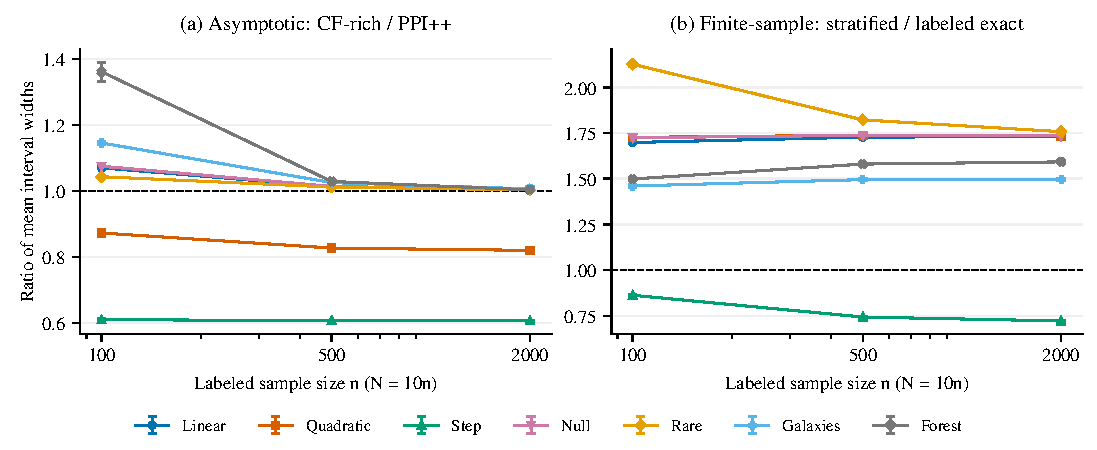
\includegraphics[width=\textwidth]{figures/efficiency/plot.pdf}
\caption{Paired mean-width ratios in all core distributions ($N=10n$), with 95\% Monte Carlo error bars. Left: nonlinear cross-fitting versus unrestricted PPI++; this is an asymptotic-tier comparison, not an assertion of matched finite-sample coverage. Right: exact two-stratum intervals versus labeled exact binomial intervals, both with finite-sample guarantees. The two panels use different references and vertical scales. Only the strongly informative fixed partition improves the exact comparator.}
\label{fig:efficiency}
\end{figure*}

\begin{table*}[t]
\centering\small
\caption{Asymptotic-tier comparison at $n=2000,N=20000$. Width ratios are ratios of mean widths against unrestricted PPI++; parentheses give paired Monte Carlo standard errors. Coverage is a fraction targeting 0.95; smaller width is preferable only subject to validity. The Step width gain accompanies an unadjusted coverage warning.}
\label{tab:asym}
\begin{tabular}{lrrrrr}
\toprule
 & \multicolumn{2}{c}{PPI++ (unrestricted)} & \multicolumn{3}{c}{Cross-fit rich} \\
Distribution & Width & Coverage & Width ratio (MC SE) & Coverage & Wilson 95\% interval \\
\midrule
Linear & 0.03933 & 0.9520 & 1.0032 (0.0001) & 0.9530 & [0.9428, 0.9614] \\
Quadratic & 0.04152 & 0.9500 & 0.8203 (0.0002) & 0.9480 & [0.9374, 0.9569] \\
Step & 0.02575 & 0.9540 & 0.6070 (0.0003) & 0.9355 & [0.9239, 0.9455] \\
Null & 0.04382 & 0.9440 & 1.0037 (0.0001) & 0.9465 & [0.9358, 0.9555] \\
Rare & 0.00865 & 0.9455 & 1.0035 (0.0001) & 0.9435 & [0.9325, 0.9528] \\
Galaxies & 0.02720 & 0.9610 & 1.0065 (0.0001) & 0.9625 & [0.9532, 0.9700] \\
Forest & 0.02698 & 0.9475 & 1.0036 (0.0001) & 0.9465 & [0.9358, 0.9555] \\
\bottomrule
\end{tabular}

\end{table*}

\cref{fig:efficiency,tab:asym} show the predicted conditional nature of score-only gains. The rich cross-fit width reductions are \QuadSaving\% for quadratic and \StepSaving\% for step at $n=2000$. The limiting width ratios from \cref{eq:widthratio} agree closely with the measured trends (analytic and empirical values are tabulated in \texttt{results/oracle.csv} and \texttt{all\_summary.csv}). The affine and null controls give no incremental improvement, while finite-dimensional fitting adds overhead. At $n=2000$, the rich method is \GalaxyIncrease\% wider for galaxies and \ForestIncrease\% wider for forest. This is evidence only about the tested basis, not proof that every nonlinear inference rule must fail on those scores.

\cref{fig:validity} summarizes the coverage failures. Width savings alone are insufficient. In the step cell at $n=2000$, rich cross-fit coverage is \StepCoverage\%, with Wilson interval [\StepCoverageLo\%,\StepCoverageHi\%]. This is an unadjusted warning, not a Holm-confirmed violation in its large test family. Even the fixed oracle normal interval can show finite-sample coverage deviations. In the rare cell at $n=30$, rich cross-fit coverage collapses to \RareCoverage\% ([\RareCoverageLo\%,\RareCoverageHi\%]); all-zero labels make the fitted correction and normal standard error vanish. Cross-fitting does not repair missing rare events. The labeled exact interval remains valid by construction. Thus these nonlinear normal intervals do \emph{not} meet a uniform finite-sample validity requirement.

\begin{figure*}[t]
\centering
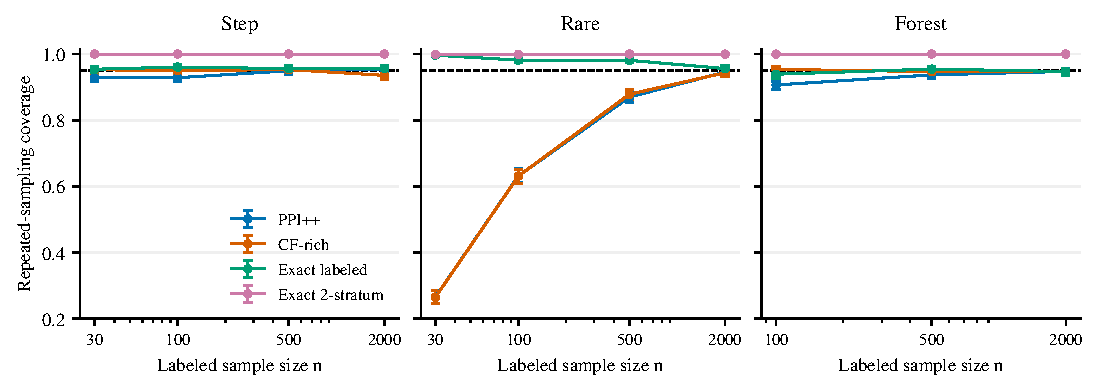
\includegraphics[width=\textwidth]{figures/validity/plot.pdf}
\caption{Coverage with Wilson 95\% Monte Carlo intervals; the dashed line is 0.95. Rare-event failures invalidate treating normal-based width gains as automatically valid. Exact procedures can be strongly conservative; reported coverage below 0.95 in an individual exact-binomial cell is sampling uncertainty, not evidence against the exact theorem. All-cell results, including unsafe in-sample fitting and oracle controls, appear in the appendix and CSVs.}
\label{fig:validity}
\end{figure*}

Across the complete screen there are \FiniteRejects\ Holm rejections among \FiniteTests\ finite-tier method-cells, versus \AsymRejects\ among \AsymTests\ asymptotic-tier method-cells. The latter family includes the deliberately unsafe in-sample negative control; it should not be read as a rejection count for PPI++ alone. Rejections are descriptive robustness diagnostics. In particular, theoretical finite-sample coverage does not imply that every Monte Carlo estimate will exceed 0.95.

\subsection{What remains under a strict finite-sample requirement?}
\begin{table*}[t]
\centering\small
\caption{Finite-sample-valid comparison at $n=2000,N=20000$. Both procedures have analytical coverage guarantees for binary outcomes under the stated iid design. The paired ratio is exact-stratified width divided by labeled-only exact-binomial width; smaller is narrower. Its Monte Carlo standard error is in parentheses. Coverage targets 0.95; no dominance across distributions is obtained.}
\label{tab:exact}
\begin{tabular}{lrrrrr}
\toprule
 & \multicolumn{2}{c}{Exact labeled binomial} & \multicolumn{3}{c}{Exact two-stratum} \\
Distribution & Width & Coverage & Width ratio (MC SE) & Coverage & Wilson 95\% interval \\
\midrule
Linear & 0.04429 & 0.9570 & 1.7315 (0.0002) & 1.0000 & [0.9981, 1.0000] \\
Quadratic & 0.04199 & 0.9535 & 1.7351 (0.0001) & 0.9995 & [0.9972, 0.9999] \\
Step & 0.04429 & 0.9560 & 0.7222 (0.0008) & 1.0000 & [0.9981, 1.0000] \\
Null & 0.04429 & 0.9490 & 1.7350 (0.0001) & 0.9990 & [0.9964, 0.9997] \\
Rare & 0.00922 & 0.9560 & 1.7579 (0.0003) & 1.0000 & [0.9981, 1.0000] \\
Galaxies & 0.03889 & 0.9510 & 1.4958 (0.0006) & 1.0000 & [0.9981, 1.0000] \\
Forest & 0.03193 & 0.9470 & 1.5925 (0.0008) & 1.0000 & [0.9981, 1.0000] \\
\bottomrule
\end{tabular}

\end{table*}

\cref{tab:exact} gives the exact-tier comparison. For the step law, exact stratification reduces mean width from \CPstepWidth\ to \ExactStepWidth, a \ExactSaving\% reduction against labeled exact binomial inference. The paired ratio is \ExactStepRatio\ (MC SE \ExactStepRatioSE), corresponding to a 95\% Monte Carlo savings interval [\ExactSavingLo\%,\ExactSavingHi\%]. Empirical coverage is 1.0000 with Wilson lower bound 0.9981; the guarantee follows from \cref{thm:exact}, not that observed coverage. In contrast, exact stratification is wider for the other six core distributions at this sample size. It improves against ordinary exact binomial inference in only three of the 32 tested cells, all step-law core cells. This fixed split cannot exploit the quadratic symmetry and incurs three simultaneous-interval penalties when the partition is unhelpful.

The Bernstein selection experiment is more negative. It reduces width by \EBstepSaving\% against labeled-only EB for the step law at $n=2000$, but is still \EBstepRatioCP\ times as wide as the exact labeled-binomial interval there. Selection correction and known-range penalties overwhelm most variance benefits; selection is wider than labeled-only EB in the other tested cells. These are failures of practical efficiency, not coverage failures. The selected interval is not guaranteed shorter than a stand-alone baseline at its own error budget. The original PPI betting-style MeanCI was not run, so this experiment cannot rank the strongest available finite-sample PPI procedures.

\subsection{Ablations and implementation checks}
Scalar cross-fitting, adding only a quadratic feature, adding the rich basis, and omitting cross-fitting are compared on identical observations in \cref{app:ablations}. The quadratic basis captures the quadratic mechanism; the rich basis, which includes a threshold feature, exactly spans the step conditional mean. The cubic and threshold features are added jointly, so this comparison cannot establish either feature's individual necessity. In-sample residuals can appear narrower because fitting reduces training errors, especially for small labeled samples; that is not valid evidence of improved uncertainty quantification. We retain these adverse comparisons rather than selecting recipes after inspecting coverage.

A separate unit test checks endpoint equality with \texttt{ppi-python==0.2.3}. Its default clips the tuning coefficient to $[0,1]$, uses a denominator-$n$ labeled covariance, and denominator-$n$ residual variances; our original-paper baseline is unrestricted, uses unbiased sample moments, and pooled score variance. The step mechanism can have an optimal coefficient exceeding one, so comparing only to the clipped implementation would overstate new-method gains. Five-fold nuisance fitting reuses the same unlabeled observations; a unit test verifies that its variance is computed with the requisite cross-fold covariances.

\section{Discussion, Limitations, and Conclusion}
The answer depends jointly on information left in the score, estimation cost, and the desired guarantee. The non-affine component of $\E[Y\mid S]$ quantifies score-only oracle opportunity after optimal scalar tuning. Learning that component is useful in favorable simulations, but normal intervals remain only asymptotically valid and can fail badly. A known-range or exact-binomial construction can supply genuine finite-sample protection without changing any input observations. Its protection can be expensive, and narrow valid intervals occur only when the fixed partition or dictionary is sufficiently informative.

Several limitations prevent a stronger conclusion. We study a bounded mean, not quantiles, regression, or arbitrary unbounded outcomes. Only two empirical paired datasets and one small predeclared feature basis are tested. With-replacement empirical experiments do not validate the original sampling designs or population representativeness. Distribution shift, dependent records, score training leakage, and a value-dependent fold assignment fall outside our assumptions. A score-only efficiency result is not an optimality theorem among procedures allowed to exploit all $X$. We also do not solve admissibility or minimax expected length, and no chosen interval is guaranteed to dominate every existing valid interval. An expensive concentration bound becoming wider is not evidence that all finite-sample inference must be equally conservative.

The restricted direct-source literature protocol is another limitation: broad novelty cannot be certified. Exact stratification and safe selection are elementary constructions from established tools. The contribution is the explicitly quantified efficiency opportunity and a reproducible guarantee-aware audit, including non-gains and failures. No post-result tuning is used to turn those failures into a universal success claim. A useful next study would validate the fixed recipes on independently chosen empirical populations and compare stronger finite-sample betting intervals, rather than optimizing hyperparameters against this simulation screen.

In conclusion, fixed data and fixed predictions do not imply that existing intervals are irreducibly wide. There can be real, finite-sample-valid shrinkage against a specified baseline, but not uniformly across the settings examined. The available room is conditional; empirical width savings from asymptotic methods must never be substituted for the nominal-coverage requirement.

\section*{Impact Statement}
Overconfident scientific intervals can turn inexpensive model predictions into unsupported claims. This study emphasizes calibration of inferential guarantees rather than unqualified precision gains. Incorrectly treating a normal approximation or an estimated stratum mass as exact can be especially harmful for rare outcomes and underrepresented strata. The work uses synthetic data and existing paired public research examples, with no new human-subject collection. The package code is MIT; a separate license for the example data was not stated in the inspected package materials, so instructions provide acquisition rather than asserting unrestricted redistribution rights. This manuscript was produced by an automated research assistant; human authorship, factual verification, and submission-policy review are necessary before any actual conference submission.

\bibliography{references}
\bibliographystyle{icml2026}

\newpage
\appendix
\onecolumn
\section{Proof Details and Assumption Audit}\label{app:proofs}
\subsection{Projection identity and its boundary cases}
For fixed $g$, independence yields
\[
nV(g)=\V(Y)-2\Cov(Y,g)+(1+r)\V(g).
\]
Write $\widetilde m=m-\E m$ and $\widetilde g=g-\E g$. Conditional expectation implies $\E[(Y-\E Y)\widetilde g]=\E[\widetilde m\widetilde g]$. Expanding
\[
(1+r)\E\left[\left(\widetilde g-\frac{\widetilde m}{1+r}\right)^2\right]
=(1+r)\V(g)-2\Cov(m,g)+\frac{\V(m)}{1+r}
\]
proves the result. The minimum is attained whenever $g-m/(1+r)$ is constant almost surely. For $\V(S)>0$, the scalar quadratic is strictly convex. Substituting its minimizer gives the excess variance in \cref{eq:gap}. The numerator is the variance of the residual in the linear projection of $m$ onto an intercept and $S$. It equals zero if and only if that residual vanishes almost surely. If $S$ is constant then $m(S)$ is constant and every score function is constant, so there is no reduction. If $\V(Y)=0$, all oracle variances vanish; a normal width ratio is then undefined and should not be used. Affine rescaling $aS+b$ with $a\ne0$ preserves the scalar correction class exactly. These facts are not assertions about arbitrary outcome-dependent confidence sets.

\subsection{Fixed-dimensional cross-fitting}
For the chosen feature subspace let $b^*$ be the population least-squares slope including an intercept, and define $g^*(s)=b^{*\top}h(s)/(1+r)$. Assume bounded $Y,h$, positive-definite feature covariance, a fixed number of folds assigned independently of observations, fold proportions bounded away from zero, $n/N\to r_0\in(0,\infty)$, and positive limiting $nV(g^*)$. The ridge coefficient rate is
\[
\|b_{-k}-b^*\|=O_p(n^{-1/2}+\epsilon_n),
\qquad\epsilon_n=10^{-4}/n_{\rm train}.
\]
Thus the implementation has root-$n$ coefficient error. More generally, consistency alone suffices for first-order equivalence here. Subtracting the fixed-control version of \cref{eq:cf} gives
\[
\frac1{1+r}\sum_k w_k(b_{-k}-b^*)^\top
\left(\bar h_U-\bar h_{L_k}\right).
\]
Every score-mean difference is $O_p(n^{-1/2})$ and the coefficient error is $o_p(1)$; a fixed number of products is $o_p(n^{-1/2})$. With the stated ridge rate this remainder is $O_p(n^{-1})$. No false independence assertion for all fitted folds is needed. The ordinary two-sample CLT for the fixed control and Slutsky's theorem then give the normal limit. Uniform convergence of the fixed-dimensional fitted controls to $g^*$, bounded features, and iid laws imply the consistency of both sample variances in \cref{eq:cfvar}.

The unlabeled term must be
\[
\frac1N\V_U\!\left(\sum_k w_k g_{-k}(T)\right),
\]
including cross-covariances. Treating the same $N$ scores as $KN$ independent observations is incorrect. Likewise, balancing folds is not sufficient if values determine assignment: sorting scores into folds can make train and held-out distributions differ. Our folds use index modulo five on iid row order before inspecting any values. These arguments give asymptotic validity with a fixed regular law. They do not give finite-sample validity, a guarantee under label shift, or uniform validity over rare-event sequences whose success probability decreases with $n$.

\subsection{Exact binomial inversion and random strata}
For $K\sim\mathrm{Bin}(m,q)$, invert equal-tail binomial tests with tail errors $\delta/2$. The lower endpoint is zero for $K=0$ and otherwise $\mathrm{Beta}^{-1}(\delta/2;K,m-K+1)$. The upper endpoint is one for $K=m$ and otherwise $\mathrm{Beta}^{-1}(1-\delta/2;K+1,m-K)$. Each rejecting tail has probability at most its allotted error by monotonicity of binomial tail probabilities. Their union therefore has probability at most $\delta$; discreteness may make the interval conservative. For $m=0$ the interval is $[0,1]$.

Conditioning on the complete labeled membership vector makes each stratum's label count binomial with its random sample size fixed. Apply the preceding guarantee conditionally and then integrate. Pooled score memberships are iid Bernoulli for the marginal $p$, regardless of their dependence on conditional-label confidence events. The union bound is valid without event independence. If a stratum has zero population mass, define its conditional mean arbitrarily in $[0,1]$; the target does not depend on it, and its interval is harmless. The bilinear target map has the extrema used in \cref{eq:strat} because its derivatives in $q_0,q_1$ are nonnegative on $p\in[0,1]$ and the resulting endpoint functions are affine in $p$.

\subsection{Empirical-Bernstein selection proof}
Normalize an observation with known range length $R>0$ to $[0,1]$. Apply the one-sided theorem of \citet{eb} at error $\delta/2$ both to the normalized variable and its complement. Rescaling gives \cref{eq:eb}, with unbiased sample variance. A nonzero dictionary member has labeled residual range $[-a,1]$ and unlabeled range $[0,a]$, hence lengths $1+a$ and $a$. Errors $\alpha/(2K)$ on each component give failure probability at most $\alpha/K$ for its sum interval. The zero control uses one component with the same total budget. A union over the $K=5$ fixed controls gives simultaneous containment with probability at least $1-\alpha$; selecting by interval width on the same observations preserves this event. The dictionary may depend on fixed sample sizes, but not on data. Intersecting with $[0,1]$ preserves containment of the true bounded mean. If a raw interval is wholly outside $[0,1]$, the implementation collapses it to the nearest endpoint; this changes only failure events and cannot remove a previously contained true mean.

\subsection{Why unbounded outcomes require extra assumptions}
The bounded-outcome restriction is substantive. Consider deterministic procedures with finite endpoints on an all-zero labeled sample and a constant zero predictor. If its upper endpoint there is $u<\infty$, choose a distribution with $Y=0$ with probability $1-\varepsilon$ and $Y=M$ with probability $\varepsilon$, where $\varepsilon M>u$. Scores remain zero. For sufficiently small $\varepsilon$, $(1-\varepsilon)^n>\alpha$, so the same all-zero observations occur with probability exceeding the permitted failure rate while the true mean exceeds the returned interval. Thus no such finite interval can guarantee $1-\alpha$ coverage uniformly over all finite-mean distributions without further restrictions. This elementary contamination example is not an impossibility result for the bounded setting or a theorem about all randomized procedures.

\section{Implementation and Reproducibility}
\paragraph{Commands.}
From the workspace root, run
\begin{verbatim}
python -m pip install -r requirements.txt
python download_data.py
export OPENBLAS_NUM_THREADS=1 OMP_NUM_THREADS=1
python -m pytest tests -q
python run_experiments.py --reps 2000 --jobs 4
python run_stratified.py --jobs 4
python analyze.py
python plot.py
latexmk -pdf -interaction=nonstopmode -halt-on-error paper.tex
\end{verbatim}
The measured main run took \RunSeconds\ seconds and the exact-stratum replay \SupplementSeconds\ seconds on the provided CPU host using four workers and single-threaded BLAS; these are whole-run wall times, not method-specific timing comparisons. Installed package versions and data hashes are in \texttt{requirements-lock.txt} and \texttt{results/config.json}. No GPU, paid API, new labels, model retraining, or prediction queries were used. The full run has 64,000 distinct repeated-sampling datasets; the supplementary replay uses the same draws, not 64,000 additional independent datasets.

\paragraph{Numerical conventions and pairing.}
All reported widths are after intersection with $[0,1]$; untruncated widths are also saved. Except for the package-matching baseline, interval variance estimates and scalar-tuning moments use denominator $m-1$ for the relevant sample size $m$. Ridge regression instead divides its training Gram and cross-moment matrices by the training sample size before adding its stated penalty. Raw endpoints are exported to 12 significant digits; summary statistics are computed before this rounding. Scenario \texttt{null} must be read with \texttt{keep\_default\_na=False}, otherwise pandas silently treats its name as missing. Sample row IDs were not saved in the primary run. Pairing follows directly from one shared input call for all procedures, and row-index alignment is audited; it is not independent evidence of stored sampling IDs. Supplemental data draws replay the same RNG call sequence. The \texttt{seconds} field in a method summary is cumulative cell elapsed time, not a per-method benchmark.

\paragraph{Failures and abandoned choices.}
The first environment check found scikit-learn absent; dependencies were then installed. A package-comparison test initially failed only because package endpoints had shape $(2,1)$ versus our shape $(2,)$; flattening the reference fixed it without changing endpoints. A plotting run failed on a negative error-bar value of floating-point roundoff magnitude at coverage one; only the visual error lengths were clamped to zero. No statistical outputs were altered. The first attempted PDF text tool was absent and a Python PDF extractor was used instead. The originally considered seven-feature hinge basis and fixed ridge were replaced by the documented four-feature basis and vanishing ridge before full results. No underlying-predictor retraining or hyperparameter search was necessary; the stated inference-nuisance regressions were fitted. The full experiment reports negative results rather than hiding recipes that fail coverage.

\paragraph{Access restrictions and conference format.}
Only direct starter-source PDFs, the original 2009 Bernstein paper, the pinned package and its dataset links, and official ICML template/instruction URLs were accessed; no topic or citation-chain search was used. No identifiable prohibited material was encountered. Since the forbidden work was not identified, undetected overlap cannot be certified absent. The code/data access log records the permitted boundaries. The latest released official ICML style located by direct URL was ICML 2026; the corresponding ICML 2027 style URL returned 404. The unmodified 2026 style and eight-page initial-submission body limit are used. The inspected ICML instructions require an impact statement, included above, but no separate NeurIPS-style paper checklist. A supplementary reproducibility checklist is included below.

\section{Ablations and Additional Results}\label{app:ablations}
\Cref{tab:ablation} reports the basis comparison; \cref{fig:allcoverage} displays every cell, and \cref{tab:full} gives complete numerical uncertainty.
\begin{table}[h]
\centering\small
\caption{Fixed-basis ablations at $n=500,N=5000$, 2000 paired repetitions. Ratios reference unrestricted PPI++; smaller width is preferable subject to coverage targeting 0.95. All recipes here are normal-based, with asymptotic assumptions for the cross-fit variants. In-sample residual fitting is an unsafe negative control, not an exact-valid baseline.}
\label{tab:ablation}
\begin{tabular}{llrrr}
\toprule
Law & Recipe & Width ratio & MC SE & Coverage \\
\midrule
Quadratic & PPI++ & 1.0000 & 0.0000 & 0.9475 \\
Quadratic & CF scalar & 1.0037 & 0.0001 & 0.9485 \\
Quadratic & CF polynomial & 0.8204 & 0.0005 & 0.9405 \\
Quadratic & CF rich & 0.8273 & 0.0005 & 0.9425 \\
Quadratic & In-sample (unsafe) & 0.8150 & 0.0005 & 0.9400 \\
Step & PPI++ & 1.0000 & 0.0000 & 0.9495 \\
Step & CF scalar & 0.9998 & 0.0000 & 0.9515 \\
Step & CF polynomial & 1.0001 & 0.0001 & 0.9485 \\
Step & CF rich & 0.6071 & 0.0007 & 0.9530 \\
Step & In-sample (unsafe) & 0.6040 & 0.0007 & 0.9535 \\
Galaxies & PPI++ & 1.0000 & 0.0000 & 0.9495 \\
Galaxies & CF scalar & 1.0005 & 0.0001 & 0.9505 \\
Galaxies & CF polynomial & 1.0002 & 0.0001 & 0.9500 \\
Galaxies & CF rich & 1.0256 & 0.0005 & 0.9525 \\
Galaxies & In-sample (unsafe) & 0.9938 & 0.0001 & 0.9465 \\
Forest & PPI++ & 1.0000 & 0.0000 & 0.9370 \\
Forest & CF scalar & 1.0013 & 0.0001 & 0.9425 \\
Forest & CF polynomial & 1.0020 & 0.0001 & 0.9415 \\
Forest & CF rich & 1.0290 & 0.0006 & 0.9470 \\
Forest & In-sample (unsafe) & 0.9888 & 0.0002 & 0.9395 \\
\bottomrule
\end{tabular}

\end{table}

\begin{figure}[p]
\centering
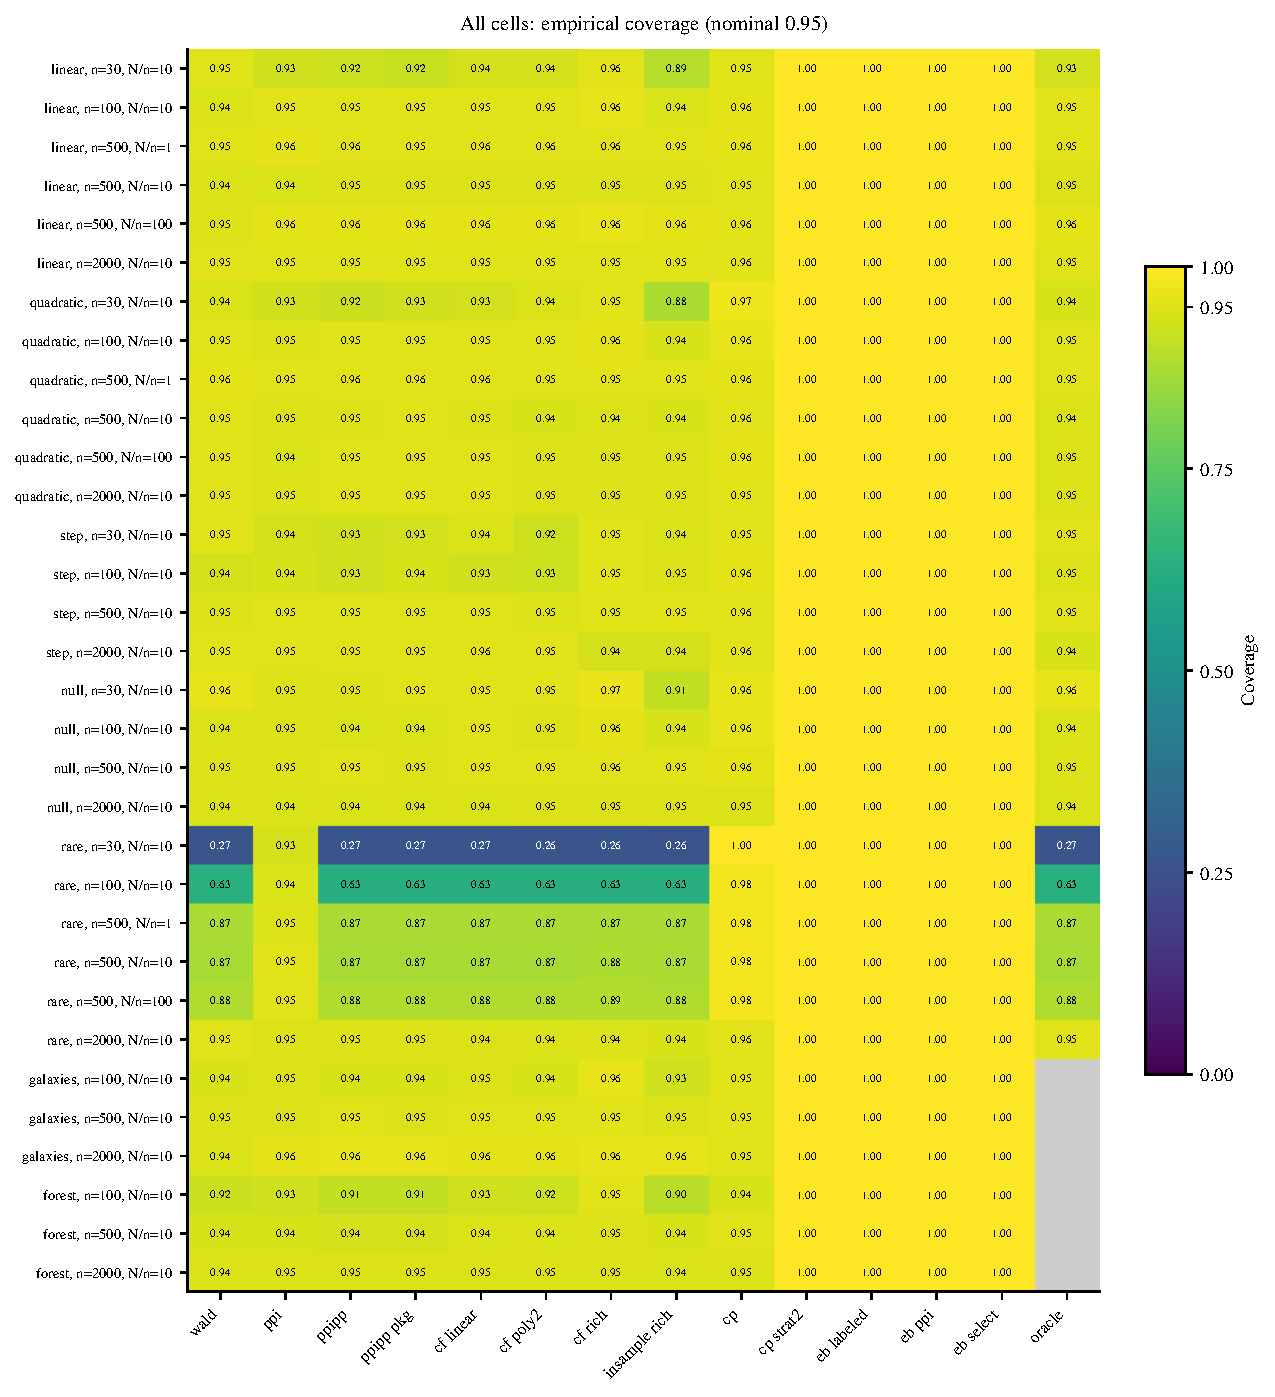
\includegraphics[width=.93\textwidth]{figures/coverage_all/plot.pdf}
\caption{All 32 cells and all interval recipes. Gray denotes unavailable real-data oracle values, not zero coverage. The color scale is $[0,1]$ and values are rounded to two decimals for display; full Wilson intervals are in the following tables and CSVs. Finite-sample guarantees belong only to the exact and Bernstein recipes under their specified assumptions.}
\label{fig:allcoverage}
\end{figure}

\section{Supplementary Reproducibility Checklist}
\begin{itemize}
\item Claims, scope and limitations: stated in the abstract, introduction and discussion; no global efficiency or priority assertion.
\item Theoretical assumptions and proofs: fixed independent predictor, common iid score law, binary or bounded labels, fixed partition/dictionary, independent folds and nondegeneracy; proofs above.
\item Data acquisition and provenance: pinned package dataset IDs and SHA-256 hashes, empirical-distribution target, no unlabeled evaluation-label leakage; data license uncertainty disclosed.
\item Experimental specification: fixed mechanisms, all sample sizes, base seed and cell streams, shared draws, folds, ridge, coefficient clipping conventions, truncation and error budgets.
\item Uncertainty: coverage Wilson intervals, width MC standard errors, paired ratio MC standard errors, and Holm-screen family definitions; no statement that simulation proves coverage.
\item Negative results: empirical non-gains, rare-outcome failures, conservative EB costs, invalid in-sample residual control, and stronger original-paper scalar baseline all included.
\item Compute and code: CPU-only commands, pinned versions, actual wall times, scripts for every table and figure, tests, saved raw outputs and plan amendments.
\item Ethics and automation: impact statement and automated-generation disclosure included. This is a research artifact, not an actual conference submission.
\end{itemize}

\section{Complete Numerical Results}
\small
\begin{longtable}{llrrrrr}
\caption{All repeated-sampling results; each row has 2000 repetitions. MC SE is the standard error of mean width; paired comparisons are additionally available in CSV.}\label{tab:full}\\
\toprule
Law, $n$, $N/n$ & Method & Coverage & Wilson lower & Wilson upper & Width & MC SE \\
\midrule\endfirsthead
\toprule Law, $n$, $N/n$ & Method & Coverage & Wilson lower & Wilson upper & Width & MC SE \\\midrule\endhead
Linear, 30, 10 & cf\_linear & 0.9365 & 0.9250 & 0.9464 & 0.32804 & 0.00070 \\
Linear, 30, 10 & cf\_poly2 & 0.9360 & 0.9244 & 0.9459 & 0.33425 & 0.00083 \\
Linear, 30, 10 & cf\_rich & 0.9565 & 0.9467 & 0.9646 & 0.41251 & 0.00181 \\
Linear, 30, 10 & cp & 0.9525 & 0.9423 & 0.9610 & 0.36813 & 0.00018 \\
Linear, 30, 10 & cp\_strat2 & 1.0000 & 0.9981 & 1.0000 & 0.58864 & 0.00065 \\
Linear, 30, 10 & eb\_labeled & 1.0000 & 0.9981 & 1.0000 & 0.98939 & 0.00064 \\
Linear, 30, 10 & eb\_ppi & 1.0000 & 0.9981 & 1.0000 & 1.00000 & 0.00000 \\
Linear, 30, 10 & eb\_select & 1.0000 & 0.9981 & 1.0000 & 0.99981 & 0.00008 \\
Linear, 30, 10 & insample\_rich & 0.8900 & 0.8755 & 0.9030 & 0.30162 & 0.00064 \\
Linear, 30, 10 & oracle & 0.9320 & 0.9201 & 0.9422 & 0.32030 & 0.00058 \\
Linear, 30, 10 & ppi & 0.9295 & 0.9174 & 0.9399 & 0.32507 & 0.00075 \\
Linear, 30, 10 & ppipp & 0.9225 & 0.9100 & 0.9334 & 0.31736 & 0.00057 \\
Linear, 30, 10 & ppipp\_pkg & 0.9170 & 0.9041 & 0.9283 & 0.31193 & 0.00057 \\
Linear, 30, 10 & wald & 0.9525 & 0.9423 & 0.9610 & 0.35739 & 0.00020 \\
Linear, 100, 10 & cf\_linear & 0.9530 & 0.9428 & 0.9614 & 0.17744 & 0.00018 \\
Linear, 100, 10 & cf\_poly2 & 0.9535 & 0.9434 & 0.9619 & 0.17810 & 0.00019 \\
Linear, 100, 10 & cf\_rich & 0.9615 & 0.9521 & 0.9691 & 0.18807 & 0.00027 \\
Linear, 100, 10 & cp & 0.9600 & 0.9505 & 0.9677 & 0.20243 & 0.00003 \\
Linear, 100, 10 & cp\_strat2 & 1.0000 & 0.9981 & 1.0000 & 0.34386 & 0.00018 \\
Linear, 100, 10 & eb\_labeled & 1.0000 & 0.9981 & 1.0000 & 0.50264 & 0.00005 \\
Linear, 100, 10 & eb\_ppi & 1.0000 & 0.9981 & 1.0000 & 0.84398 & 0.00040 \\
Linear, 100, 10 & eb\_select & 1.0000 & 0.9981 & 1.0000 & 0.62864 & 0.00005 \\
Linear, 100, 10 & insample\_rich & 0.9425 & 0.9314 & 0.9519 & 0.17326 & 0.00017 \\
Linear, 100, 10 & oracle & 0.9545 & 0.9445 & 0.9628 & 0.17619 & 0.00017 \\
Linear, 100, 10 & ppi & 0.9545 & 0.9445 & 0.9628 & 0.17913 & 0.00022 \\
Linear, 100, 10 & ppipp & 0.9505 & 0.9401 & 0.9592 & 0.17570 & 0.00017 \\
Linear, 100, 10 & ppipp\_pkg & 0.9495 & 0.9390 & 0.9583 & 0.17483 & 0.00017 \\
Linear, 100, 10 & wald & 0.9430 & 0.9320 & 0.9523 & 0.19602 & 0.00003 \\
Linear, 500, 1 & cf\_linear & 0.9560 & 0.9461 & 0.9641 & 0.08289 & 0.00002 \\
Linear, 500, 1 & cf\_poly2 & 0.9555 & 0.9456 & 0.9637 & 0.08291 & 0.00002 \\
Linear, 500, 1 & cf\_rich & 0.9560 & 0.9461 & 0.9641 & 0.08319 & 0.00002 \\
Linear, 500, 1 & cp & 0.9590 & 0.9494 & 0.9668 & 0.08935 & 0.00000 \\
Linear, 500, 1 & cp\_strat2 & 1.0000 & 0.9981 & 1.0000 & 0.17167 & 0.00001 \\
Linear, 500, 1 & eb\_labeled & 1.0000 & 0.9981 & 1.0000 & 0.17338 & 0.00000 \\
Linear, 500, 1 & eb\_ppi & 1.0000 & 0.9981 & 1.0000 & 0.35204 & 0.00008 \\
Linear, 500, 1 & eb\_select & 1.0000 & 0.9981 & 1.0000 & 0.21085 & 0.00000 \\
Linear, 500, 1 & insample\_rich & 0.9545 & 0.9445 & 0.9628 & 0.08271 & 0.00002 \\
Linear, 500, 1 & oracle & 0.9535 & 0.9434 & 0.9619 & 0.08285 & 0.00002 \\
Linear, 500, 1 & ppi & 0.9580 & 0.9483 & 0.9659 & 0.09331 & 0.00004 \\
Linear, 500, 1 & ppipp & 0.9555 & 0.9456 & 0.9637 & 0.08282 & 0.00002 \\
Linear, 500, 1 & ppipp\_pkg & 0.9550 & 0.9450 & 0.9632 & 0.08273 & 0.00002 \\
Linear, 500, 1 & wald & 0.9510 & 0.9406 & 0.9596 & 0.08766 & 0.00000 \\
Linear, 500, 10 & cf\_linear & 0.9475 & 0.9368 & 0.9564 & 0.07877 & 0.00003 \\
Linear, 500, 10 & cf\_poly2 & 0.9470 & 0.9363 & 0.9560 & 0.07883 & 0.00003 \\
Linear, 500, 10 & cf\_rich & 0.9485 & 0.9379 & 0.9574 & 0.07964 & 0.00004 \\
Linear, 500, 10 & cp & 0.9530 & 0.9428 & 0.9614 & 0.08934 & 0.00000 \\
Linear, 500, 10 & cp\_strat2 & 1.0000 & 0.9981 & 1.0000 & 0.15438 & 0.00003 \\
Linear, 500, 10 & eb\_labeled & 0.9995 & 0.9972 & 0.9999 & 0.17337 & 0.00000 \\
Linear, 500, 10 & eb\_ppi & 1.0000 & 0.9981 & 1.0000 & 0.25305 & 0.00007 \\
Linear, 500, 10 & eb\_select & 1.0000 & 0.9981 & 1.0000 & 0.21084 & 0.00001 \\
Linear, 500, 10 & insample\_rich & 0.9455 & 0.9347 & 0.9546 & 0.07841 & 0.00003 \\
Linear, 500, 10 & oracle & 0.9480 & 0.9374 & 0.9569 & 0.07867 & 0.00003 \\
Linear, 500, 10 & ppi & 0.9435 & 0.9325 & 0.9528 & 0.07998 & 0.00004 \\
Linear, 500, 10 & ppipp & 0.9470 & 0.9363 & 0.9560 & 0.07863 & 0.00003 \\
Linear, 500, 10 & ppipp\_pkg & 0.9465 & 0.9358 & 0.9555 & 0.07855 & 0.00003 \\
Linear, 500, 10 & wald & 0.9425 & 0.9314 & 0.9519 & 0.08765 & 0.00000 \\
Linear, 500, 100 & cf\_linear & 0.9580 & 0.9483 & 0.9659 & 0.07800 & 0.00004 \\
Linear, 500, 100 & cf\_poly2 & 0.9595 & 0.9499 & 0.9673 & 0.07806 & 0.00004 \\
Linear, 500, 100 & cf\_rich & 0.9615 & 0.9521 & 0.9691 & 0.07905 & 0.00004 \\
Linear, 500, 100 & cp & 0.9570 & 0.9472 & 0.9650 & 0.08935 & 0.00000 \\
Linear, 500, 100 & cp\_strat2 & 1.0000 & 0.9981 & 1.0000 & 0.14588 & 0.00005 \\
Linear, 500, 100 & eb\_labeled & 1.0000 & 0.9981 & 1.0000 & 0.17338 & 0.00000 \\
Linear, 500, 100 & eb\_ppi & 1.0000 & 0.9981 & 1.0000 & 0.23113 & 0.00007 \\
Linear, 500, 100 & eb\_select & 1.0000 & 0.9981 & 1.0000 & 0.21085 & 0.00000 \\
Linear, 500, 100 & insample\_rich & 0.9580 & 0.9483 & 0.9659 & 0.07760 & 0.00004 \\
Linear, 500, 100 & oracle & 0.9580 & 0.9483 & 0.9659 & 0.07788 & 0.00004 \\
Linear, 500, 100 & ppi & 0.9585 & 0.9488 & 0.9664 & 0.07860 & 0.00004 \\
Linear, 500, 100 & ppipp & 0.9575 & 0.9477 & 0.9655 & 0.07784 & 0.00004 \\
Linear, 500, 100 & ppipp\_pkg & 0.9575 & 0.9477 & 0.9655 & 0.07776 & 0.00004 \\
Linear, 500, 100 & wald & 0.9490 & 0.9385 & 0.9578 & 0.08766 & 0.00000 \\
Linear, 2000, 10 & cf\_linear & 0.9525 & 0.9423 & 0.9610 & 0.03935 & 0.00001 \\
Linear, 2000, 10 & cf\_poly2 & 0.9515 & 0.9412 & 0.9601 & 0.03936 & 0.00001 \\
Linear, 2000, 10 & cf\_rich & 0.9530 & 0.9428 & 0.9614 & 0.03946 & 0.00001 \\
Linear, 2000, 10 & cp & 0.9570 & 0.9472 & 0.9650 & 0.04429 & 0.00000 \\
Linear, 2000, 10 & cp\_strat2 & 1.0000 & 0.9981 & 1.0000 & 0.07669 & 0.00001 \\
Linear, 2000, 10 & eb\_labeled & 1.0000 & 0.9981 & 1.0000 & 0.07643 & 0.00000 \\
Linear, 2000, 10 & eb\_ppi & 1.0000 & 0.9981 & 1.0000 & 0.10159 & 0.00002 \\
Linear, 2000, 10 & eb\_select & 1.0000 & 0.9981 & 1.0000 & 0.09139 & 0.00000 \\
Linear, 2000, 10 & insample\_rich & 0.9520 & 0.9417 & 0.9605 & 0.03931 & 0.00001 \\
Linear, 2000, 10 & oracle & 0.9520 & 0.9417 & 0.9605 & 0.03934 & 0.00001 \\
Linear, 2000, 10 & ppi & 0.9495 & 0.9390 & 0.9583 & 0.04000 & 0.00001 \\
Linear, 2000, 10 & ppipp & 0.9520 & 0.9417 & 0.9605 & 0.03933 & 0.00001 \\
Linear, 2000, 10 & ppipp\_pkg & 0.9520 & 0.9417 & 0.9605 & 0.03932 & 0.00001 \\
Linear, 2000, 10 & wald & 0.9540 & 0.9439 & 0.9623 & 0.04383 & 0.00000 \\
Quadratic, 30, 10 & cf\_linear & 0.9305 & 0.9185 & 0.9408 & 0.35223 & 0.00072 \\
Quadratic, 30, 10 & cf\_poly2 & 0.9445 & 0.9336 & 0.9537 & 0.29613 & 0.00096 \\
Quadratic, 30, 10 & cf\_rich & 0.9530 & 0.9428 & 0.9614 & 0.35302 & 0.00165 \\
Quadratic, 30, 10 & cp & 0.9730 & 0.9649 & 0.9792 & 0.35049 & 0.00048 \\
Quadratic, 30, 10 & cp\_strat2 & 1.0000 & 0.9981 & 1.0000 & 0.57911 & 0.00078 \\
Quadratic, 30, 10 & eb\_labeled & 1.0000 & 0.9981 & 1.0000 & 0.92669 & 0.00178 \\
Quadratic, 30, 10 & eb\_ppi & 1.0000 & 0.9981 & 1.0000 & 1.00000 & 0.00000 \\
Quadratic, 30, 10 & eb\_select & 1.0000 & 0.9981 & 1.0000 & 0.99185 & 0.00059 \\
Quadratic, 30, 10 & insample\_rich & 0.8780 & 0.8629 & 0.8916 & 0.26007 & 0.00076 \\
Quadratic, 30, 10 & oracle & 0.9385 & 0.9271 & 0.9482 & 0.27486 & 0.00075 \\
Quadratic, 30, 10 & ppi & 0.9290 & 0.9169 & 0.9395 & 0.39622 & 0.00113 \\
Quadratic, 30, 10 & ppipp & 0.9180 & 0.9052 & 0.9292 & 0.33007 & 0.00060 \\
Quadratic, 30, 10 & ppipp\_pkg & 0.9260 & 0.9137 & 0.9367 & 0.32811 & 0.00057 \\
Quadratic, 30, 10 & wald & 0.9450 & 0.9341 & 0.9542 & 0.33779 & 0.00054 \\
Quadratic, 100, 10 & cf\_linear & 0.9550 & 0.9450 & 0.9632 & 0.18783 & 0.00016 \\
Quadratic, 100, 10 & cf\_poly2 & 0.9505 & 0.9401 & 0.9592 & 0.15427 & 0.00024 \\
Quadratic, 100, 10 & cf\_rich & 0.9585 & 0.9488 & 0.9664 & 0.16095 & 0.00030 \\
Quadratic, 100, 10 & cp & 0.9635 & 0.9544 & 0.9709 & 0.19226 & 0.00014 \\
Quadratic, 100, 10 & cp\_strat2 & 0.9995 & 0.9972 & 0.9999 & 0.33195 & 0.00025 \\
Quadratic, 100, 10 & eb\_labeled & 1.0000 & 0.9981 & 1.0000 & 0.48672 & 0.00023 \\
Quadratic, 100, 10 & eb\_ppi & 1.0000 & 0.9981 & 1.0000 & 0.79620 & 0.00143 \\
Quadratic, 100, 10 & eb\_select & 1.0000 & 0.9981 & 1.0000 & 0.60572 & 0.00048 \\
Quadratic, 100, 10 & insample\_rich & 0.9400 & 0.9287 & 0.9496 & 0.14917 & 0.00022 \\
Quadratic, 100, 10 & oracle & 0.9495 & 0.9390 & 0.9583 & 0.15144 & 0.00022 \\
Quadratic, 100, 10 & ppi & 0.9465 & 0.9358 & 0.9555 & 0.21996 & 0.00030 \\
Quadratic, 100, 10 & ppipp & 0.9495 & 0.9390 & 0.9583 & 0.18437 & 0.00015 \\
Quadratic, 100, 10 & ppipp\_pkg & 0.9505 & 0.9401 & 0.9592 & 0.18402 & 0.00015 \\
Quadratic, 100, 10 & wald & 0.9520 & 0.9417 & 0.9605 & 0.18554 & 0.00015 \\
Quadratic, 500, 1 & cf\_linear & 0.9560 & 0.9461 & 0.9641 & 0.08312 & 0.00003 \\
Quadratic, 500, 1 & cf\_poly2 & 0.9530 & 0.9428 & 0.9614 & 0.07519 & 0.00003 \\
Quadratic, 500, 1 & cf\_rich & 0.9535 & 0.9434 & 0.9619 & 0.07537 & 0.00003 \\
Quadratic, 500, 1 & cp & 0.9605 & 0.9510 & 0.9682 & 0.08476 & 0.00003 \\
Quadratic, 500, 1 & cp\_strat2 & 0.9985 & 0.9956 & 0.9995 & 0.14873 & 0.00006 \\
Quadratic, 500, 1 & eb\_labeled & 0.9990 & 0.9964 & 0.9997 & 0.16641 & 0.00004 \\
Quadratic, 500, 1 & eb\_ppi & 1.0000 & 0.9981 & 1.0000 & 0.38273 & 0.00011 \\
Quadratic, 500, 1 & eb\_select & 1.0000 & 0.9981 & 1.0000 & 0.20269 & 0.00005 \\
Quadratic, 500, 1 & insample\_rich & 0.9515 & 0.9412 & 0.9601 & 0.07499 & 0.00003 \\
Quadratic, 500, 1 & oracle & 0.9505 & 0.9401 & 0.9592 & 0.07509 & 0.00003 \\
Quadratic, 500, 1 & ppi & 0.9525 & 0.9423 & 0.9610 & 0.10964 & 0.00006 \\
Quadratic, 500, 1 & ppipp & 0.9555 & 0.9456 & 0.9637 & 0.08298 & 0.00003 \\
Quadratic, 500, 1 & ppipp\_pkg & 0.9570 & 0.9472 & 0.9650 & 0.08293 & 0.00003 \\
Quadratic, 500, 1 & wald & 0.9575 & 0.9477 & 0.9655 & 0.08304 & 0.00003 \\
Quadratic, 500, 10 & cf\_linear & 0.9485 & 0.9379 & 0.9574 & 0.08327 & 0.00003 \\
Quadratic, 500, 10 & cf\_poly2 & 0.9405 & 0.9293 & 0.9500 & 0.06806 & 0.00005 \\
Quadratic, 500, 10 & cf\_rich & 0.9425 & 0.9314 & 0.9519 & 0.06864 & 0.00005 \\
Quadratic, 500, 10 & cp & 0.9565 & 0.9467 & 0.9646 & 0.08479 & 0.00003 \\
Quadratic, 500, 10 & cp\_strat2 & 0.9995 & 0.9972 & 0.9999 & 0.14740 & 0.00005 \\
Quadratic, 500, 10 & eb\_labeled & 1.0000 & 0.9981 & 1.0000 & 0.16645 & 0.00004 \\
Quadratic, 500, 10 & eb\_ppi & 1.0000 & 0.9981 & 1.0000 & 0.28364 & 0.00010 \\
Quadratic, 500, 10 & eb\_select & 1.0000 & 0.9981 & 1.0000 & 0.20274 & 0.00005 \\
Quadratic, 500, 10 & insample\_rich & 0.9400 & 0.9287 & 0.9496 & 0.06762 & 0.00004 \\
Quadratic, 500, 10 & oracle & 0.9440 & 0.9330 & 0.9533 & 0.06782 & 0.00004 \\
Quadratic, 500, 10 & ppi & 0.9485 & 0.9379 & 0.9574 & 0.09849 & 0.00006 \\
Quadratic, 500, 10 & ppipp & 0.9475 & 0.9368 & 0.9564 & 0.08297 & 0.00003 \\
Quadratic, 500, 10 & ppipp\_pkg & 0.9510 & 0.9406 & 0.9596 & 0.08293 & 0.00003 \\
Quadratic, 500, 10 & wald & 0.9515 & 0.9412 & 0.9601 & 0.08307 & 0.00003 \\
Quadratic, 500, 100 & cf\_linear & 0.9535 & 0.9434 & 0.9619 & 0.08329 & 0.00003 \\
Quadratic, 500, 100 & cf\_poly2 & 0.9470 & 0.9363 & 0.9560 & 0.06670 & 0.00005 \\
Quadratic, 500, 100 & cf\_rich & 0.9490 & 0.9385 & 0.9578 & 0.06737 & 0.00005 \\
Quadratic, 500, 100 & cp & 0.9595 & 0.9499 & 0.9673 & 0.08479 & 0.00003 \\
Quadratic, 500, 100 & cp\_strat2 & 0.9995 & 0.9972 & 0.9999 & 0.14669 & 0.00005 \\
Quadratic, 500, 100 & eb\_labeled & 0.9995 & 0.9972 & 0.9999 & 0.16646 & 0.00004 \\
Quadratic, 500, 100 & eb\_ppi & 1.0000 & 0.9981 & 1.0000 & 0.26165 & 0.00010 \\
Quadratic, 500, 100 & eb\_select & 1.0000 & 0.9981 & 1.0000 & 0.20275 & 0.00005 \\
Quadratic, 500, 100 & insample\_rich & 0.9460 & 0.9352 & 0.9551 & 0.06621 & 0.00005 \\
Quadratic, 500, 100 & oracle & 0.9470 & 0.9363 & 0.9560 & 0.06642 & 0.00005 \\
Quadratic, 500, 100 & ppi & 0.9430 & 0.9320 & 0.9523 & 0.09735 & 0.00006 \\
Quadratic, 500, 100 & ppipp & 0.9530 & 0.9428 & 0.9614 & 0.08296 & 0.00003 \\
Quadratic, 500, 100 & ppipp\_pkg & 0.9540 & 0.9439 & 0.9623 & 0.08293 & 0.00003 \\
Quadratic, 500, 100 & wald & 0.9550 & 0.9450 & 0.9632 & 0.08307 & 0.00003 \\
Quadratic, 2000, 10 & cf\_linear & 0.9500 & 0.9396 & 0.9587 & 0.04156 & 0.00001 \\
Quadratic, 2000, 10 & cf\_poly2 & 0.9480 & 0.9374 & 0.9569 & 0.03399 & 0.00001 \\
Quadratic, 2000, 10 & cf\_rich & 0.9480 & 0.9374 & 0.9569 & 0.03406 & 0.00001 \\
Quadratic, 2000, 10 & cp & 0.9535 & 0.9434 & 0.9619 & 0.04199 & 0.00001 \\
Quadratic, 2000, 10 & cp\_strat2 & 0.9995 & 0.9972 & 0.9999 & 0.07287 & 0.00001 \\
Quadratic, 2000, 10 & eb\_labeled & 0.9995 & 0.9972 & 0.9999 & 0.07296 & 0.00001 \\
Quadratic, 2000, 10 & eb\_ppi & 1.0000 & 0.9981 & 1.0000 & 0.11691 & 0.00002 \\
Quadratic, 2000, 10 & eb\_select & 1.0000 & 0.9981 & 1.0000 & 0.08734 & 0.00001 \\
Quadratic, 2000, 10 & insample\_rich & 0.9485 & 0.9379 & 0.9574 & 0.03393 & 0.00001 \\
Quadratic, 2000, 10 & oracle & 0.9475 & 0.9368 & 0.9564 & 0.03396 & 0.00001 \\
Quadratic, 2000, 10 & ppi & 0.9485 & 0.9379 & 0.9574 & 0.04927 & 0.00001 \\
Quadratic, 2000, 10 & ppipp & 0.9500 & 0.9396 & 0.9587 & 0.04152 & 0.00001 \\
Quadratic, 2000, 10 & ppipp\_pkg & 0.9500 & 0.9396 & 0.9587 & 0.04151 & 0.00001 \\
Quadratic, 2000, 10 & wald & 0.9505 & 0.9401 & 0.9592 & 0.04153 & 0.00001 \\
Step, 30, 10 & cf\_linear & 0.9415 & 0.9303 & 0.9510 & 0.21243 & 0.00055 \\
Step, 30, 10 & cf\_poly2 & 0.9225 & 0.9100 & 0.9334 & 0.21841 & 0.00076 \\
Step, 30, 10 & cf\_rich & 0.9525 & 0.9423 & 0.9610 & 0.13272 & 0.00106 \\
Step, 30, 10 & cp & 0.9540 & 0.9439 & 0.9623 & 0.36824 & 0.00018 \\
Step, 30, 10 & cp\_strat2 & 1.0000 & 0.9981 & 1.0000 & 0.38863 & 0.00054 \\
Step, 30, 10 & eb\_labeled & 1.0000 & 0.9981 & 1.0000 & 0.98988 & 0.00061 \\
Step, 30, 10 & eb\_ppi & 1.0000 & 0.9981 & 1.0000 & 1.00000 & 0.00000 \\
Step, 30, 10 & eb\_select & 1.0000 & 0.9981 & 1.0000 & 0.99989 & 0.00005 \\
Step, 30, 10 & insample\_rich & 0.9415 & 0.9303 & 0.9510 & 0.12205 & 0.00056 \\
Step, 30, 10 & oracle & 0.9540 & 0.9439 & 0.9623 & 0.12385 & 0.00063 \\
Step, 30, 10 & ppi & 0.9370 & 0.9255 & 0.9468 & 0.22185 & 0.00045 \\
Step, 30, 10 & ppipp & 0.9295 & 0.9174 & 0.9399 & 0.21274 & 0.00049 \\
Step, 30, 10 & ppipp\_pkg & 0.9315 & 0.9196 & 0.9418 & 0.21853 & 0.00044 \\
Step, 30, 10 & wald & 0.9540 & 0.9439 & 0.9623 & 0.35752 & 0.00020 \\
Step, 100, 10 & cf\_linear & 0.9290 & 0.9169 & 0.9395 & 0.11527 & 0.00016 \\
Step, 100, 10 & cf\_poly2 & 0.9255 & 0.9132 & 0.9362 & 0.11551 & 0.00016 \\
Step, 100, 10 & cf\_rich & 0.9500 & 0.9396 & 0.9587 & 0.07044 & 0.00024 \\
Step, 100, 10 & cp & 0.9605 & 0.9510 & 0.9682 & 0.20237 & 0.00003 \\
Step, 100, 10 & cp\_strat2 & 1.0000 & 0.9981 & 1.0000 & 0.17457 & 0.00034 \\
Step, 100, 10 & eb\_labeled & 1.0000 & 0.9981 & 1.0000 & 0.50255 & 0.00005 \\
Step, 100, 10 & eb\_ppi & 1.0000 & 0.9981 & 1.0000 & 0.74933 & 0.00023 \\
Step, 100, 10 & eb\_select & 1.0000 & 0.9981 & 1.0000 & 0.62853 & 0.00006 \\
Step, 100, 10 & insample\_rich & 0.9470 & 0.9363 & 0.9560 & 0.06870 & 0.00020 \\
Step, 100, 10 & oracle & 0.9480 & 0.9374 & 0.9569 & 0.06905 & 0.00021 \\
Step, 100, 10 & ppi & 0.9390 & 0.9276 & 0.9487 & 0.12166 & 0.00013 \\
Step, 100, 10 & ppipp & 0.9285 & 0.9164 & 0.9390 & 0.11535 & 0.00015 \\
Step, 100, 10 & ppipp\_pkg & 0.9380 & 0.9266 & 0.9478 & 0.12109 & 0.00013 \\
Step, 100, 10 & wald & 0.9360 & 0.9244 & 0.9459 & 0.19596 & 0.00003 \\
Step, 500, 10 & cf\_linear & 0.9515 & 0.9412 & 0.9601 & 0.05149 & 0.00003 \\
Step, 500, 10 & cf\_poly2 & 0.9485 & 0.9379 & 0.9574 & 0.05150 & 0.00003 \\
Step, 500, 10 & cf\_rich & 0.9530 & 0.9428 & 0.9614 & 0.03127 & 0.00004 \\
Step, 500, 10 & cp & 0.9560 & 0.9461 & 0.9641 & 0.08934 & 0.00000 \\
Step, 500, 10 & cp\_strat2 & 1.0000 & 0.9981 & 1.0000 & 0.06643 & 0.00013 \\
Step, 500, 10 & eb\_labeled & 1.0000 & 0.9981 & 1.0000 & 0.17338 & 0.00000 \\
Step, 500, 10 & eb\_ppi & 1.0000 & 0.9981 & 1.0000 & 0.21031 & 0.00005 \\
Step, 500, 10 & eb\_select & 1.0000 & 0.9981 & 1.0000 & 0.20511 & 0.00012 \\
Step, 500, 10 & insample\_rich & 0.9535 & 0.9434 & 0.9619 & 0.03110 & 0.00004 \\
Step, 500, 10 & oracle & 0.9535 & 0.9434 & 0.9619 & 0.03114 & 0.00004 \\
Step, 500, 10 & ppi & 0.9505 & 0.9401 & 0.9592 & 0.05447 & 0.00003 \\
Step, 500, 10 & ppipp & 0.9495 & 0.9390 & 0.9583 & 0.05150 & 0.00003 \\
Step, 500, 10 & ppipp\_pkg & 0.9505 & 0.9401 & 0.9592 & 0.05442 & 0.00003 \\
Step, 500, 10 & wald & 0.9470 & 0.9363 & 0.9560 & 0.08765 & 0.00000 \\
Step, 2000, 10 & cf\_linear & 0.9560 & 0.9461 & 0.9641 & 0.02575 & 0.00001 \\
Step, 2000, 10 & cf\_poly2 & 0.9545 & 0.9445 & 0.9628 & 0.02575 & 0.00001 \\
Step, 2000, 10 & cf\_rich & 0.9355 & 0.9239 & 0.9455 & 0.01563 & 0.00001 \\
Step, 2000, 10 & cp & 0.9560 & 0.9461 & 0.9641 & 0.04429 & 0.00000 \\
Step, 2000, 10 & cp\_strat2 & 1.0000 & 0.9981 & 1.0000 & 0.03198 & 0.00003 \\
Step, 2000, 10 & eb\_labeled & 1.0000 & 0.9981 & 1.0000 & 0.07643 & 0.00000 \\
Step, 2000, 10 & eb\_ppi & 1.0000 & 0.9981 & 1.0000 & 0.08023 & 0.00001 \\
Step, 2000, 10 & eb\_select & 1.0000 & 0.9981 & 1.0000 & 0.07195 & 0.00003 \\
Step, 2000, 10 & insample\_rich & 0.9370 & 0.9255 & 0.9468 & 0.01561 & 0.00001 \\
Step, 2000, 10 & oracle & 0.9385 & 0.9271 & 0.9482 & 0.01562 & 0.00001 \\
Step, 2000, 10 & ppi & 0.9500 & 0.9396 & 0.9587 & 0.02725 & 0.00001 \\
Step, 2000, 10 & ppipp & 0.9540 & 0.9439 & 0.9623 & 0.02575 & 0.00001 \\
Step, 2000, 10 & ppipp\_pkg & 0.9500 & 0.9396 & 0.9587 & 0.02724 & 0.00001 \\
Step, 2000, 10 & wald & 0.9510 & 0.9406 & 0.9596 & 0.04383 & 0.00000 \\
Null, 30, 10 & cf\_linear & 0.9530 & 0.9428 & 0.9614 & 0.36938 & 0.00045 \\
Null, 30, 10 & cf\_poly2 & 0.9515 & 0.9412 & 0.9601 & 0.38114 & 0.00067 \\
Null, 30, 10 & cf\_rich & 0.9710 & 0.9627 & 0.9775 & 0.46709 & 0.00185 \\
Null, 30, 10 & cp & 0.9620 & 0.9527 & 0.9695 & 0.36871 & 0.00017 \\
Null, 30, 10 & cp\_strat2 & 1.0000 & 0.9981 & 1.0000 & 0.60724 & 0.00034 \\
Null, 30, 10 & eb\_labeled & 1.0000 & 0.9981 & 1.0000 & 0.99144 & 0.00056 \\
Null, 30, 10 & eb\_ppi & 1.0000 & 0.9981 & 1.0000 & 1.00000 & 0.00000 \\
Null, 30, 10 & eb\_select & 1.0000 & 0.9981 & 1.0000 & 0.99990 & 0.00005 \\
Null, 30, 10 & insample\_rich & 0.9095 & 0.8961 & 0.9213 & 0.33474 & 0.00038 \\
Null, 30, 10 & oracle & 0.9620 & 0.9527 & 0.9695 & 0.35804 & 0.00018 \\
Null, 30, 10 & ppi & 0.9455 & 0.9347 & 0.9546 & 0.41762 & 0.00078 \\
Null, 30, 10 & ppipp & 0.9480 & 0.9374 & 0.9569 & 0.35243 & 0.00025 \\
Null, 30, 10 & ppipp\_pkg & 0.9515 & 0.9412 & 0.9601 & 0.34930 & 0.00023 \\
Null, 30, 10 & wald & 0.9620 & 0.9527 & 0.9695 & 0.35804 & 0.00018 \\
Null, 100, 10 & cf\_linear & 0.9515 & 0.9412 & 0.9601 & 0.19772 & 0.00007 \\
Null, 100, 10 & cf\_poly2 & 0.9485 & 0.9379 & 0.9574 & 0.19916 & 0.00009 \\
Null, 100, 10 & cf\_rich & 0.9575 & 0.9477 & 0.9655 & 0.20979 & 0.00023 \\
Null, 100, 10 & cp & 0.9630 & 0.9538 & 0.9704 & 0.20240 & 0.00003 \\
Null, 100, 10 & cp\_strat2 & 0.9990 & 0.9964 & 0.9997 & 0.34908 & 0.00008 \\
Null, 100, 10 & eb\_labeled & 1.0000 & 0.9981 & 1.0000 & 0.50260 & 0.00005 \\
Null, 100, 10 & eb\_ppi & 1.0000 & 0.9981 & 1.0000 & 0.90838 & 0.00069 \\
Null, 100, 10 & eb\_select & 1.0000 & 0.9981 & 1.0000 & 0.62858 & 0.00006 \\
Null, 100, 10 & insample\_rich & 0.9380 & 0.9266 & 0.9478 & 0.19240 & 0.00006 \\
Null, 100, 10 & oracle & 0.9420 & 0.9309 & 0.9514 & 0.19599 & 0.00003 \\
Null, 100, 10 & ppi & 0.9460 & 0.9352 & 0.9551 & 0.22850 & 0.00022 \\
Null, 100, 10 & ppipp & 0.9445 & 0.9336 & 0.9537 & 0.19512 & 0.00004 \\
Null, 100, 10 & ppipp\_pkg & 0.9420 & 0.9309 & 0.9514 & 0.19455 & 0.00004 \\
Null, 100, 10 & wald & 0.9420 & 0.9309 & 0.9514 & 0.19599 & 0.00003 \\
Null, 500, 10 & cf\_linear & 0.9505 & 0.9401 & 0.9592 & 0.08780 & 0.00001 \\
Null, 500, 10 & cf\_poly2 & 0.9515 & 0.9412 & 0.9601 & 0.08793 & 0.00001 \\
Null, 500, 10 & cf\_rich & 0.9560 & 0.9461 & 0.9641 & 0.08880 & 0.00002 \\
Null, 500, 10 & cp & 0.9580 & 0.9483 & 0.9659 & 0.08934 & 0.00000 \\
Null, 500, 10 & cp\_strat2 & 1.0000 & 0.9981 & 1.0000 & 0.15528 & 0.00002 \\
Null, 500, 10 & eb\_labeled & 1.0000 & 0.9981 & 1.0000 & 0.17338 & 0.00000 \\
Null, 500, 10 & eb\_ppi & 1.0000 & 0.9981 & 1.0000 & 0.29020 & 0.00007 \\
Null, 500, 10 & eb\_select & 1.0000 & 0.9981 & 1.0000 & 0.21085 & 0.00000 \\
Null, 500, 10 & insample\_rich & 0.9520 & 0.9417 & 0.9605 & 0.08734 & 0.00001 \\
Null, 500, 10 & oracle & 0.9485 & 0.9379 & 0.9574 & 0.08765 & 0.00000 \\
Null, 500, 10 & ppi & 0.9490 & 0.9385 & 0.9578 & 0.10248 & 0.00004 \\
Null, 500, 10 & ppipp & 0.9500 & 0.9396 & 0.9587 & 0.08758 & 0.00000 \\
Null, 500, 10 & ppipp\_pkg & 0.9490 & 0.9385 & 0.9578 & 0.08753 & 0.00000 \\
Null, 500, 10 & wald & 0.9485 & 0.9379 & 0.9574 & 0.08765 & 0.00000 \\
Null, 2000, 10 & cf\_linear & 0.9435 & 0.9325 & 0.9528 & 0.04385 & 0.00000 \\
Null, 2000, 10 & cf\_poly2 & 0.9460 & 0.9352 & 0.9551 & 0.04386 & 0.00000 \\
Null, 2000, 10 & cf\_rich & 0.9465 & 0.9358 & 0.9555 & 0.04398 & 0.00000 \\
Null, 2000, 10 & cp & 0.9490 & 0.9385 & 0.9578 & 0.04429 & 0.00000 \\
Null, 2000, 10 & cp\_strat2 & 0.9990 & 0.9964 & 0.9997 & 0.07684 & 0.00000 \\
Null, 2000, 10 & eb\_labeled & 0.9990 & 0.9964 & 0.9997 & 0.07643 & 0.00000 \\
Null, 2000, 10 & eb\_ppi & 1.0000 & 0.9981 & 1.0000 & 0.12011 & 0.00002 \\
Null, 2000, 10 & eb\_select & 1.0000 & 0.9981 & 1.0000 & 0.09139 & 0.00000 \\
Null, 2000, 10 & insample\_rich & 0.9455 & 0.9347 & 0.9546 & 0.04379 & 0.00000 \\
Null, 2000, 10 & oracle & 0.9425 & 0.9314 & 0.9519 & 0.04383 & 0.00000 \\
Null, 2000, 10 & ppi & 0.9445 & 0.9336 & 0.9537 & 0.05121 & 0.00001 \\
Null, 2000, 10 & ppipp & 0.9440 & 0.9330 & 0.9533 & 0.04382 & 0.00000 \\
Null, 2000, 10 & ppipp\_pkg & 0.9435 & 0.9325 & 0.9528 & 0.04381 & 0.00000 \\
Null, 2000, 10 & wald & 0.9425 & 0.9314 & 0.9519 & 0.04383 & 0.00000 \\
Rare, 30, 10 & cf\_linear & 0.2650 & 0.2461 & 0.2848 & 0.02918 & 0.00112 \\
Rare, 30, 10 & cf\_poly2 & 0.2645 & 0.2456 & 0.2843 & 0.02964 & 0.00114 \\
Rare, 30, 10 & cf\_rich & 0.2645 & 0.2456 & 0.2843 & 0.03408 & 0.00134 \\
Rare, 30, 10 & cp & 0.9965 & 0.9928 & 0.9983 & 0.13213 & 0.00064 \\
Rare, 30, 10 & cp\_strat2 & 0.9985 & 0.9956 & 0.9995 & 0.30026 & 0.00070 \\
Rare, 30, 10 & eb\_labeled & 1.0000 & 0.9981 & 1.0000 & 0.39053 & 0.00145 \\
Rare, 30, 10 & eb\_ppi & 1.0000 & 0.9981 & 1.0000 & 0.99770 & 0.00023 \\
Rare, 30, 10 & eb\_select & 1.0000 & 0.9981 & 1.0000 & 0.52472 & 0.00162 \\
Rare, 30, 10 & insample\_rich & 0.2560 & 0.2374 & 0.2756 & 0.02695 & 0.00104 \\
Rare, 30, 10 & oracle & 0.2655 & 0.2466 & 0.2853 & 0.02858 & 0.00110 \\
Rare, 30, 10 & ppi & 0.9340 & 0.9223 & 0.9441 & 0.12223 & 0.00135 \\
Rare, 30, 10 & ppipp & 0.2650 & 0.2461 & 0.2848 & 0.02841 & 0.00109 \\
Rare, 30, 10 & ppipp\_pkg & 0.2655 & 0.2466 & 0.2853 & 0.02824 & 0.00108 \\
Rare, 30, 10 & wald & 0.2655 & 0.2466 & 0.2853 & 0.02858 & 0.00110 \\
Rare, 100, 10 & cf\_linear & 0.6315 & 0.6101 & 0.6524 & 0.02512 & 0.00049 \\
Rare, 100, 10 & cf\_poly2 & 0.6315 & 0.6101 & 0.6524 & 0.02518 & 0.00049 \\
Rare, 100, 10 & cf\_rich & 0.6310 & 0.6096 & 0.6519 & 0.02600 & 0.00051 \\
Rare, 100, 10 & cp & 0.9815 & 0.9746 & 0.9865 & 0.05226 & 0.00032 \\
Rare, 100, 10 & cp\_strat2 & 0.9990 & 0.9964 & 0.9997 & 0.11117 & 0.00040 \\
Rare, 100, 10 & eb\_labeled & 1.0000 & 0.9981 & 1.0000 & 0.13601 & 0.00063 \\
Rare, 100, 10 & eb\_ppi & 1.0000 & 0.9981 & 1.0000 & 0.38725 & 0.00077 \\
Rare, 100, 10 & eb\_select & 1.0000 & 0.9981 & 1.0000 & 0.17780 & 0.00070 \\
Rare, 100, 10 & insample\_rich & 0.6305 & 0.6091 & 0.6514 & 0.02462 & 0.00048 \\
Rare, 100, 10 & oracle & 0.6330 & 0.6116 & 0.6538 & 0.02498 & 0.00049 \\
Rare, 100, 10 & ppi & 0.9425 & 0.9314 & 0.9519 & 0.07178 & 0.00070 \\
Rare, 100, 10 & ppipp & 0.6315 & 0.6101 & 0.6524 & 0.02492 & 0.00049 \\
Rare, 100, 10 & ppipp\_pkg & 0.6320 & 0.6106 & 0.6529 & 0.02486 & 0.00048 \\
Rare, 100, 10 & wald & 0.6330 & 0.6116 & 0.6538 & 0.02498 & 0.00049 \\
Rare, 500, 1 & cf\_linear & 0.8720 & 0.8566 & 0.8859 & 0.01655 & 0.00010 \\
Rare, 500, 1 & cf\_poly2 & 0.8720 & 0.8566 & 0.8859 & 0.01656 & 0.00010 \\
Rare, 500, 1 & cf\_rich & 0.8735 & 0.8582 & 0.8874 & 0.01662 & 0.00010 \\
Rare, 500, 1 & cp & 0.9810 & 0.9740 & 0.9861 & 0.01940 & 0.00008 \\
Rare, 500, 1 & cp\_strat2 & 1.0000 & 0.9981 & 1.0000 & 0.03564 & 0.00013 \\
Rare, 500, 1 & eb\_labeled & 1.0000 & 0.9981 & 1.0000 & 0.04307 & 0.00016 \\
Rare, 500, 1 & eb\_ppi & 1.0000 & 0.9981 & 1.0000 & 0.16577 & 0.00042 \\
Rare, 500, 1 & eb\_select & 1.0000 & 0.9981 & 1.0000 & 0.05275 & 0.00017 \\
Rare, 500, 1 & insample\_rich & 0.8725 & 0.8572 & 0.8864 & 0.01651 & 0.00010 \\
Rare, 500, 1 & oracle & 0.8715 & 0.8561 & 0.8855 & 0.01654 & 0.00010 \\
Rare, 500, 1 & ppi & 0.9465 & 0.9358 & 0.9555 & 0.04624 & 0.00039 \\
Rare, 500, 1 & ppipp & 0.8720 & 0.8566 & 0.8859 & 0.01654 & 0.00010 \\
Rare, 500, 1 & ppipp\_pkg & 0.8720 & 0.8566 & 0.8859 & 0.01652 & 0.00010 \\
Rare, 500, 1 & wald & 0.8715 & 0.8561 & 0.8855 & 0.01654 & 0.00010 \\
Rare, 500, 10 & cf\_linear & 0.8705 & 0.8551 & 0.8845 & 0.01669 & 0.00010 \\
Rare, 500, 10 & cf\_poly2 & 0.8710 & 0.8556 & 0.8850 & 0.01671 & 0.00010 \\
Rare, 500, 10 & cf\_rich & 0.8785 & 0.8635 & 0.8921 & 0.01686 & 0.00010 \\
Rare, 500, 10 & cp & 0.9810 & 0.9740 & 0.9861 & 0.01952 & 0.00009 \\
Rare, 500, 10 & cp\_strat2 & 1.0000 & 0.9981 & 1.0000 & 0.03557 & 0.00013 \\
Rare, 500, 10 & eb\_labeled & 1.0000 & 0.9981 & 1.0000 & 0.04333 & 0.00017 \\
Rare, 500, 10 & eb\_ppi & 1.0000 & 0.9981 & 1.0000 & 0.11638 & 0.00032 \\
Rare, 500, 10 & eb\_select & 1.0000 & 0.9981 & 1.0000 & 0.05302 & 0.00018 \\
Rare, 500, 10 & insample\_rich & 0.8730 & 0.8577 & 0.8869 & 0.01661 & 0.00010 \\
Rare, 500, 10 & oracle & 0.8695 & 0.8540 & 0.8836 & 0.01667 & 0.00010 \\
Rare, 500, 10 & ppi & 0.9545 & 0.9445 & 0.9628 & 0.03738 & 0.00029 \\
Rare, 500, 10 & ppipp & 0.8700 & 0.8545 & 0.8840 & 0.01665 & 0.00010 \\
Rare, 500, 10 & ppipp\_pkg & 0.8695 & 0.8540 & 0.8836 & 0.01665 & 0.00010 \\
Rare, 500, 10 & wald & 0.8695 & 0.8540 & 0.8836 & 0.01667 & 0.00010 \\
Rare, 500, 100 & cf\_linear & 0.8805 & 0.8655 & 0.8940 & 0.01683 & 0.00010 \\
Rare, 500, 100 & cf\_poly2 & 0.8805 & 0.8655 & 0.8940 & 0.01685 & 0.00010 \\
Rare, 500, 100 & cf\_rich & 0.8855 & 0.8708 & 0.8987 & 0.01702 & 0.00010 \\
Rare, 500, 100 & cp & 0.9835 & 0.9769 & 0.9882 & 0.01962 & 0.00008 \\
Rare, 500, 100 & cp\_strat2 & 1.0000 & 0.9981 & 1.0000 & 0.03556 & 0.00013 \\
Rare, 500, 100 & eb\_labeled & 1.0000 & 0.9981 & 1.0000 & 0.04351 & 0.00016 \\
Rare, 500, 100 & eb\_ppi & 1.0000 & 0.9981 & 1.0000 & 0.10546 & 0.00031 \\
Rare, 500, 100 & eb\_select & 1.0000 & 0.9981 & 1.0000 & 0.05322 & 0.00018 \\
Rare, 500, 100 & insample\_rich & 0.8810 & 0.8661 & 0.8945 & 0.01673 & 0.00010 \\
Rare, 500, 100 & oracle & 0.8800 & 0.8650 & 0.8935 & 0.01680 & 0.00010 \\
Rare, 500, 100 & ppi & 0.9550 & 0.9450 & 0.9632 & 0.03635 & 0.00027 \\
Rare, 500, 100 & ppipp & 0.8805 & 0.8655 & 0.8940 & 0.01678 & 0.00010 \\
Rare, 500, 100 & ppipp\_pkg & 0.8800 & 0.8650 & 0.8935 & 0.01678 & 0.00010 \\
Rare, 500, 100 & wald & 0.8800 & 0.8650 & 0.8935 & 0.01680 & 0.00010 \\
Rare, 2000, 10 & cf\_linear & 0.9450 & 0.9341 & 0.9542 & 0.00866 & 0.00002 \\
Rare, 2000, 10 & cf\_poly2 & 0.9440 & 0.9330 & 0.9533 & 0.00866 & 0.00002 \\
Rare, 2000, 10 & cf\_rich & 0.9435 & 0.9325 & 0.9528 & 0.00868 & 0.00002 \\
Rare, 2000, 10 & cp & 0.9560 & 0.9461 & 0.9641 & 0.00922 & 0.00002 \\
Rare, 2000, 10 & cp\_strat2 & 1.0000 & 0.9981 & 1.0000 & 0.01620 & 0.00004 \\
Rare, 2000, 10 & eb\_labeled & 1.0000 & 0.9981 & 1.0000 & 0.02150 & 0.00006 \\
Rare, 2000, 10 & eb\_ppi & 1.0000 & 0.9981 & 1.0000 & 0.05074 & 0.00016 \\
Rare, 2000, 10 & eb\_select & 1.0000 & 0.9981 & 1.0000 & 0.02460 & 0.00007 \\
Rare, 2000, 10 & insample\_rich & 0.9390 & 0.9276 & 0.9487 & 0.00865 & 0.00002 \\
Rare, 2000, 10 & oracle & 0.9500 & 0.9396 & 0.9587 & 0.00865 & 0.00002 \\
Rare, 2000, 10 & ppi & 0.9485 & 0.9379 & 0.9574 & 0.02273 & 0.00012 \\
Rare, 2000, 10 & ppipp & 0.9455 & 0.9347 & 0.9546 & 0.00865 & 0.00002 \\
Rare, 2000, 10 & ppipp\_pkg & 0.9470 & 0.9363 & 0.9560 & 0.00865 & 0.00002 \\
Rare, 2000, 10 & wald & 0.9500 & 0.9396 & 0.9587 & 0.00865 & 0.00002 \\
Galaxies, 100, 10 & cf\_linear & 0.9475 & 0.9368 & 0.9564 & 0.12145 & 0.00027 \\
Galaxies, 100, 10 & cf\_poly2 & 0.9405 & 0.9293 & 0.9500 & 0.12131 & 0.00028 \\
Galaxies, 100, 10 & cf\_rich & 0.9620 & 0.9527 & 0.9695 & 0.13880 & 0.00042 \\
Galaxies, 100, 10 & cp & 0.9550 & 0.9450 & 0.9632 & 0.17842 & 0.00021 \\
Galaxies, 100, 10 & cp\_strat2 & 1.0000 & 0.9981 & 1.0000 & 0.26058 & 0.00045 \\
Galaxies, 100, 10 & eb\_labeled & 1.0000 & 0.9981 & 1.0000 & 0.46019 & 0.00056 \\
Galaxies, 100, 10 & eb\_ppi & 1.0000 & 0.9981 & 1.0000 & 0.63579 & 0.00082 \\
Galaxies, 100, 10 & eb\_select & 1.0000 & 0.9981 & 1.0000 & 0.54708 & 0.00105 \\
Galaxies, 100, 10 & insample\_rich & 0.9270 & 0.9148 & 0.9376 & 0.11734 & 0.00028 \\
Galaxies, 100, 10 & ppi & 0.9470 & 0.9363 & 0.9560 & 0.12149 & 0.00028 \\
Galaxies, 100, 10 & ppipp & 0.9390 & 0.9276 & 0.9487 & 0.12115 & 0.00026 \\
Galaxies, 100, 10 & ppipp\_pkg & 0.9380 & 0.9266 & 0.9478 & 0.12025 & 0.00026 \\
Galaxies, 100, 10 & wald & 0.9395 & 0.9282 & 0.9491 & 0.17125 & 0.00022 \\
Galaxies, 500, 10 & cf\_linear & 0.9505 & 0.9401 & 0.9592 & 0.05444 & 0.00005 \\
Galaxies, 500, 10 & cf\_poly2 & 0.9500 & 0.9396 & 0.9587 & 0.05442 & 0.00005 \\
Galaxies, 500, 10 & cf\_rich & 0.9525 & 0.9423 & 0.9610 & 0.05580 & 0.00006 \\
Galaxies, 500, 10 & cp & 0.9550 & 0.9450 & 0.9632 & 0.07850 & 0.00004 \\
Galaxies, 500, 10 & cp\_strat2 & 1.0000 & 0.9981 & 1.0000 & 0.11741 & 0.00009 \\
Galaxies, 500, 10 & eb\_labeled & 1.0000 & 0.9981 & 1.0000 & 0.15690 & 0.00006 \\
Galaxies, 500, 10 & eb\_ppi & 1.0000 & 0.9981 & 1.0000 & 0.21347 & 0.00009 \\
Galaxies, 500, 10 & eb\_select & 1.0000 & 0.9981 & 1.0000 & 0.19158 & 0.00008 \\
Galaxies, 500, 10 & insample\_rich & 0.9465 & 0.9358 & 0.9555 & 0.05407 & 0.00005 \\
Galaxies, 500, 10 & ppi & 0.9490 & 0.9385 & 0.9578 & 0.05480 & 0.00006 \\
Galaxies, 500, 10 & ppipp & 0.9495 & 0.9390 & 0.9583 & 0.05441 & 0.00005 \\
Galaxies, 500, 10 & ppipp\_pkg & 0.9485 & 0.9379 & 0.9574 & 0.05435 & 0.00005 \\
Galaxies, 500, 10 & wald & 0.9485 & 0.9379 & 0.9574 & 0.07675 & 0.00004 \\
Galaxies, 2000, 10 & cf\_linear & 0.9605 & 0.9510 & 0.9682 & 0.02720 & 0.00001 \\
Galaxies, 2000, 10 & cf\_poly2 & 0.9605 & 0.9510 & 0.9682 & 0.02720 & 0.00001 \\
Galaxies, 2000, 10 & cf\_rich & 0.9625 & 0.9532 & 0.9700 & 0.02738 & 0.00001 \\
Galaxies, 2000, 10 & cp & 0.9510 & 0.9406 & 0.9596 & 0.03889 & 0.00001 \\
Galaxies, 2000, 10 & cp\_strat2 & 1.0000 & 0.9981 & 1.0000 & 0.05816 & 0.00002 \\
Galaxies, 2000, 10 & eb\_labeled & 1.0000 & 0.9981 & 1.0000 & 0.06825 & 0.00002 \\
Galaxies, 2000, 10 & eb\_ppi & 1.0000 & 0.9981 & 1.0000 & 0.08180 & 0.00002 \\
Galaxies, 2000, 10 & eb\_select & 1.0000 & 0.9981 & 1.0000 & 0.08183 & 0.00002 \\
Galaxies, 2000, 10 & insample\_rich & 0.9615 & 0.9521 & 0.9691 & 0.02716 & 0.00001 \\
Galaxies, 2000, 10 & ppi & 0.9600 & 0.9505 & 0.9677 & 0.02740 & 0.00001 \\
Galaxies, 2000, 10 & ppipp & 0.9610 & 0.9516 & 0.9686 & 0.02720 & 0.00001 \\
Galaxies, 2000, 10 & ppipp\_pkg & 0.9610 & 0.9516 & 0.9686 & 0.02720 & 0.00001 \\
Galaxies, 2000, 10 & wald & 0.9440 & 0.9330 & 0.9533 & 0.03842 & 0.00001 \\
Forest, 100, 10 & cf\_linear & 0.9270 & 0.9148 & 0.9376 & 0.12149 & 0.00032 \\
Forest, 100, 10 & cf\_poly2 & 0.9240 & 0.9116 & 0.9348 & 0.12456 & 0.00047 \\
Forest, 100, 10 & cf\_rich & 0.9535 & 0.9434 & 0.9619 & 0.16390 & 0.00180 \\
Forest, 100, 10 & cp & 0.9390 & 0.9276 & 0.9487 & 0.14787 & 0.00032 \\
Forest, 100, 10 & cp\_strat2 & 1.0000 & 0.9981 & 1.0000 & 0.22166 & 0.00043 \\
Forest, 100, 10 & eb\_labeled & 1.0000 & 0.9981 & 1.0000 & 0.35971 & 0.00107 \\
Forest, 100, 10 & eb\_ppi & 1.0000 & 0.9981 & 1.0000 & 0.51929 & 0.00093 \\
Forest, 100, 10 & eb\_select & 1.0000 & 0.9981 & 1.0000 & 0.41586 & 0.00113 \\
Forest, 100, 10 & insample\_rich & 0.8960 & 0.8819 & 0.9086 & 0.11553 & 0.00036 \\
Forest, 100, 10 & ppi & 0.9265 & 0.9142 & 0.9371 & 0.12102 & 0.00033 \\
Forest, 100, 10 & ppipp & 0.9065 & 0.8929 & 0.9185 & 0.12039 & 0.00032 \\
Forest, 100, 10 & ppipp\_pkg & 0.9070 & 0.8935 & 0.9190 & 0.11913 & 0.00032 \\
Forest, 100, 10 & wald & 0.9180 & 0.9052 & 0.9292 & 0.13964 & 0.00033 \\
Forest, 500, 10 & cf\_linear & 0.9425 & 0.9314 & 0.9519 & 0.05412 & 0.00006 \\
Forest, 500, 10 & cf\_poly2 & 0.9415 & 0.9303 & 0.9510 & 0.05416 & 0.00006 \\
Forest, 500, 10 & cf\_rich & 0.9470 & 0.9363 & 0.9560 & 0.05562 & 0.00007 \\
Forest, 500, 10 & cp & 0.9545 & 0.9445 & 0.9628 & 0.06471 & 0.00006 \\
Forest, 500, 10 & cp\_strat2 & 1.0000 & 0.9981 & 1.0000 & 0.10228 & 0.00009 \\
Forest, 500, 10 & eb\_labeled & 1.0000 & 0.9981 & 1.0000 & 0.13593 & 0.00009 \\
Forest, 500, 10 & eb\_ppi & 1.0000 & 0.9981 & 1.0000 & 0.20546 & 0.00011 \\
Forest, 500, 10 & eb\_select & 1.0000 & 0.9981 & 1.0000 & 0.16706 & 0.00011 \\
Forest, 500, 10 & insample\_rich & 0.9395 & 0.9282 & 0.9491 & 0.05345 & 0.00006 \\
Forest, 500, 10 & ppi & 0.9405 & 0.9293 & 0.9500 & 0.05450 & 0.00006 \\
Forest, 500, 10 & ppipp & 0.9370 & 0.9255 & 0.9468 & 0.05405 & 0.00006 \\
Forest, 500, 10 & ppipp\_pkg & 0.9355 & 0.9239 & 0.9455 & 0.05398 & 0.00006 \\
Forest, 500, 10 & wald & 0.9385 & 0.9271 & 0.9482 & 0.06286 & 0.00006 \\
Forest, 2000, 10 & cf\_linear & 0.9470 & 0.9363 & 0.9560 & 0.02699 & 0.00002 \\
Forest, 2000, 10 & cf\_poly2 & 0.9465 & 0.9358 & 0.9555 & 0.02699 & 0.00002 \\
Forest, 2000, 10 & cf\_rich & 0.9465 & 0.9358 & 0.9555 & 0.02708 & 0.00002 \\
Forest, 2000, 10 & cp & 0.9470 & 0.9363 & 0.9560 & 0.03193 & 0.00002 \\
Forest, 2000, 10 & cp\_strat2 & 1.0000 & 0.9981 & 1.0000 & 0.05085 & 0.00002 \\
Forest, 2000, 10 & eb\_labeled & 0.9995 & 0.9972 & 0.9999 & 0.05773 & 0.00002 \\
Forest, 2000, 10 & eb\_ppi & 1.0000 & 0.9981 & 1.0000 & 0.07773 & 0.00003 \\
Forest, 2000, 10 & eb\_select & 1.0000 & 0.9981 & 1.0000 & 0.06953 & 0.00003 \\
Forest, 2000, 10 & insample\_rich & 0.9445 & 0.9336 & 0.9537 & 0.02682 & 0.00001 \\
Forest, 2000, 10 & ppi & 0.9480 & 0.9374 & 0.9569 & 0.02722 & 0.00002 \\
Forest, 2000, 10 & ppipp & 0.9475 & 0.9368 & 0.9564 & 0.02698 & 0.00002 \\
Forest, 2000, 10 & ppipp\_pkg & 0.9470 & 0.9363 & 0.9560 & 0.02697 & 0.00002 \\
Forest, 2000, 10 & wald & 0.9440 & 0.9330 & 0.9533 & 0.03145 & 0.00002 \\
\bottomrule
\end{longtable}


\end{document}
